\documentclass[12pt,a4paper]{article}

\usepackage[a4paper,margin=1in]{geometry}
\usepackage{graphicx}
\usepackage{booktabs}
\usepackage{amsmath,amssymb}
\usepackage{float}
\usepackage{hyperref}
\usepackage{xcolor}
\usepackage{listings}
\usepackage{enumitem}
\usepackage{fancyhdr}
\usepackage{longtable}
\usepackage{subcaption}

\hypersetup{colorlinks=true,linkcolor=blue,urlcolor=blue,citecolor=blue}

\pagestyle{fancy}
\fancyhf{}
\lhead{ICS1512 - Machine Learning Algorithms Laboratory}
\rhead{Experiment 6 / 7}
\cfoot{\thepage}

\lstset{
language=Python,
basicstyle=\ttfamily\small,
numbers=left,
frame=single,
breaklines=true,
showstringspaces=false,
keywordstyle=\color{blue},
commentstyle=\color{gray},
stringstyle=\color{red}
}

\begin{document}

\begin{center}
\Large\bfseries SRI SIVASUBRAMANIYA NADAR COLLEGE OF ENGINEERING, CHENNAI\\
\small (An Autonomous Institution Affiliated to Anna University)\\
\vspace{0.2cm}
\large\bfseries Department of Computer Science and Engineering\\
\large B.E. Computer Science and Engineering -- VI Semester\\
\vspace{0.3cm}
\large\bfseries ICS1512 -- Machine Learning Laboratory\\
\vspace{0.4cm}
\Large\bfseries EXPERIMENT REPORT\\
\vspace{0.2cm}
\large Bagging, Boosting, and Stacked Ensemble Models
\end{center}

\vspace{0.3cm}

\begin{table}[H]
\centering
\begin{tabular}{|p{4.2cm}|p{10.8cm}|}
\hline
\textbf{Experiment No.} & 6 / 7 \\ \hline
\textbf{Experiment Title} & Bagging, Boosting, and Stacked Ensemble Models \\ \hline
\textbf{GitHub Repository} & \href{https://github.com/rishirithesh/ML_Lab}{https://github.com/rishirithesh/ML\_Lab} \\ \hline
\textbf{Student Name} & Rishi Rithesh \\ \hline
\textbf{Register Number} & 3122247001049 \\ \hline
\textbf{Faculty} & Dr. Poreddy Ajay Kumar Reddy \\ \hline
\textbf{Academic Year} & 2026--2027 (Even) / Batch: 2024--2029 \\ \hline
\end{tabular}
\end{table}

\section{Objective}
\begin{itemize}[leftmargin=*]
    \item To understand the theoretical foundations and operational mechanics of primary ensemble learning paradigms: \textbf{Bagging} (Bootstrap Aggregation), \textbf{Boosting} (Adaptive Boosting and Gradient Tree Boosting), and \textbf{Stacking} (Stacked Generalization).
    \item To implement a \textbf{Bagging Classifier} with Decision Tree base estimators and analyze the influence of bootstrap sample fractions and number of estimators.
    \item To implement and evaluate sequential \textbf{Boosting Classifiers} (\texttt{AdaBoostClassifier} and \texttt{GradientBoostingClassifier}) with systematically tuned learning rates, estimator counts, and tree depths.
    \item To construct a heterogeneous \textbf{Stacked Ensemble Model} integrating Support Vector Machines (SVM), Gaussian Na\"ive Bayes, and Decision Trees via a Logistic Regression meta-learner.
    \item To benchmark ensemble models against individual base classifiers across standard evaluation metrics (Accuracy, Precision, Recall, F1-Score, ROC-AUC, Confusion Matrices, and PR Curves).
    \item To perform 5-fold Stratified Cross-Validation for unbiased hyperparameter selection and performance validation.
    \item To empirically decompose prediction errors into \textbf{Bias and Variance} components, verifying theoretical reduction characteristics.
\end{itemize}

\section{Problem Statement}
\begin{description}
    \item[Problem:] To classify breast tumors as either \textit{Malignant} or \textit{Benign} based on cytological attributes extracted from Fine Needle Aspirate (FNA) digitized microscopic biopsy images, comparing how Bagging, Boosting, and Stacking improve predictive reliability, generalization capacity, and stability compared to single baseline learners.
    \item[Input:] Wisconsin Diagnostic Breast Cancer (WDBC) dataset comprising 569 clinical biopsy records characterized by 30 continuous morphometric features describing nuclear size, shape, texture, and boundary irregularities.
    \item[Output:] Cleaned and standardized feature matrices, comprehensive Exploratory Data Analysis (EDA) visualizations, hyperparameter optimization tables (Tables 1, 2, and 3), comprehensive benchmark table (Table 4), multi-model confusion matrices, ROC/PR curves, feature importances, empirical bias-variance decomposition plots, and detailed analytical answers to observation questions.
\end{description}

\section{Dataset Description}
The Wisconsin Diagnostic Breast Cancer (WDBC) dataset is a standard medical diagnostic benchmark repository maintained by the University of California, Irvine (UCI) and University of Wisconsin Hospitals.

\begin{table}[H]
\centering
\caption{Wisconsin Diagnostic Breast Cancer (WDBC) Dataset Characteristics}
\label{tab:dataset_summary}
\begin{tabular}{|p{6cm}|p{8cm}|}
\hline
\textbf{Attribute} & \textbf{Value / Specification} \\ \hline
Dataset Name & Wisconsin Diagnostic Breast Cancer (WDBC) \\ \hline
Dataset Source & UCI ML Repository / \texttt{sklearn.datasets} \\ \hline
Total Samples ($N$) & 569 patient biopsy cases \\ \hline
Total Feature Attributes & 30 continuous cytological descriptors \\ \hline
Morphological Metrics Computed & Radius, Texture, Perimeter, Area, Smoothness, Compactness, Concavity, Concave Points, Symmetry, Fractal Dimension \\ \hline
Statistical Aggregations & Mean, Standard Error (SE), and "Worst" (mean of 3 largest values) for each metric \\ \hline
Target Variable & \texttt{diagnosis} (Binary: Malignant / Benign) \\ \hline
Class Distribution & Benign (B): 357 (62.74\%), Malignant (M): 212 (37.26\%) \\ \hline
Missing Values & 0 missing records across all features \\ \hline
Data Partitioning & 80\% Training (455 samples), 20\% Testing (114 samples) using Stratified Split \\ \hline
\end{tabular}
\end{table}

\section{Theoretical Background}

\subsection{Bagging (Bootstrap Aggregation)}
Bagging is a parallel ensemble paradigm designed to reduce the \textbf{variance} of high-capacity, low-bias estimators (such as fully grown Decision Trees) without altering their bias.
\begin{enumerate}
    \item Given training set $\mathcal{D} = \{(\mathbf{x}_i, y_i)\}_{i=1}^N$, $M$ bootstrap datasets $\mathcal{D}_1, \dots, \mathcal{D}_M$ of size $N$ are generated by uniform sampling with replacement:
    \begin{equation}
    P(\mathbf{x}_i \in \mathcal{D}_m) = 1 - \left(1 - \frac{1}{N}\right)^N \approx 1 - \frac{1}{e} \approx 63.2\%
    \end{equation}
    \item Base estimators $h_m(\mathbf{x})$ are trained independently on $\mathcal{D}_m$.
    \item Predictions are combined via majority hard voting:
    \begin{equation}
    \hat{H}_{\text{bag}}(\mathbf{x}) = \operatorname{mode}\Big(\{h_1(\mathbf{x}), h_2(\mathbf{x}), \dots, h_M(\mathbf{x})\}\Big)
    \end{equation}
\end{enumerate}

\textbf{Mathematical Variance Reduction:} If each base model has variance $\sigma^2$ and positive pairwise correlation $\rho$, the ensemble variance satisfies:
\begin{equation}
\text{Var}\left(\frac{1}{M}\sum_{m=1}^M h_m(\mathbf{x})\right) = \rho \sigma^2 + \frac{1 - \rho}{M} \sigma^2
\end{equation}
As $M \to \infty$, the second term approaches zero, bounding ensemble variance strictly to $\rho \sigma^2 < \sigma^2$.

\subsection{Boosting}
Boosting is a sequential ensemble method designed primarily to reduce \textbf{bias} by iteratively training weak learners on sample distributions reweighted according to residual errors.

\subsubsection{AdaBoost (Adaptive Boosting)}
AdaBoost maintains sample weights $w_i^{(m)}$. At step $m$, with weighted classification error $\epsilon_m = \sum_{i: y_i \neq h_m(\mathbf{x}_i)} w_i^{(m)} / \sum_i w_i^{(m)}$, the estimator coefficient is:
\begin{equation}
\alpha_m = \frac{1}{2} \ln \left( \frac{1 - \epsilon_m}{\epsilon_m} \right)
\end{equation}
Sample weights are updated exponentially:
\begin{equation}
w_i^{(m+1)} = w_i^{(m)} \exp\left(-\alpha_m y_i h_m(\mathbf{x}_i)\right)
\end{equation}

\subsubsection{Gradient Tree Boosting}
Gradient Boosting formulates ensemble construction as numerical functional gradient descent in loss space. At stage $m$, trees fit the pseudo-residuals $r_{im}$:
\begin{equation}
r_{im} = -\left[ \frac{\partial L(y_i, f(\mathbf{x}_i))}{\partial f(\mathbf{x}_i)} \right]_{f(\mathbf{x}) = f_{m-1}(\mathbf{x})}
\end{equation}
With shrinkage rate $\eta \in (0, 1]$, the updated ensemble predictor is:
\begin{equation}
f_m(\mathbf{x}) = f_{m-1}(\mathbf{x}) + \eta \sum_{j=1}^{J_m} \gamma_{jm} \mathbb{I}(\mathbf{x} \in R_{jm})
\end{equation}

\subsection{Stacked Ensemble (Stacking)}
Stacking combines heterogeneous base learners exhibiting distinct inductive biases. In this experiment:
\begin{itemize}
    \item \textbf{Base Learner 1 (SVM):} Maximizes geometric separation margin using non-linear Radial Basis Function (RBF) kernel mapping.
    \item \textbf{Base Learner 2 (Gaussian Na\"ive Bayes):} Computes class posterior probabilities under feature conditional independence.
    \item \textbf{Base Learner 3 (Decision Tree):} Constructs non-parametric axis-aligned orthogonal feature space partitions.
    \item \textbf{Meta-Learner (Logistic Regression):} Learns optimal blending coefficients $w_1, w_2, w_3$ on out-of-fold probability predictions $\mathbf{Z} \in \mathbb{R}^{N \times 3}$:
    \begin{equation}
    P(y=1 \mid \mathbf{x}) = \sigma\left(w_0 + w_1 \hat{p}_{\text{SVM}}(\mathbf{x}) + w_2 \hat{p}_{\text{NB}}(\mathbf{x}) + w_3 \hat{p}_{\text{DT}}(\mathbf{x})\right)
    \end{equation}
\end{itemize}

\section{Exploratory Data Analysis}

\subsection{Class Distribution Analysis}
\begin{figure}[H]
\centering
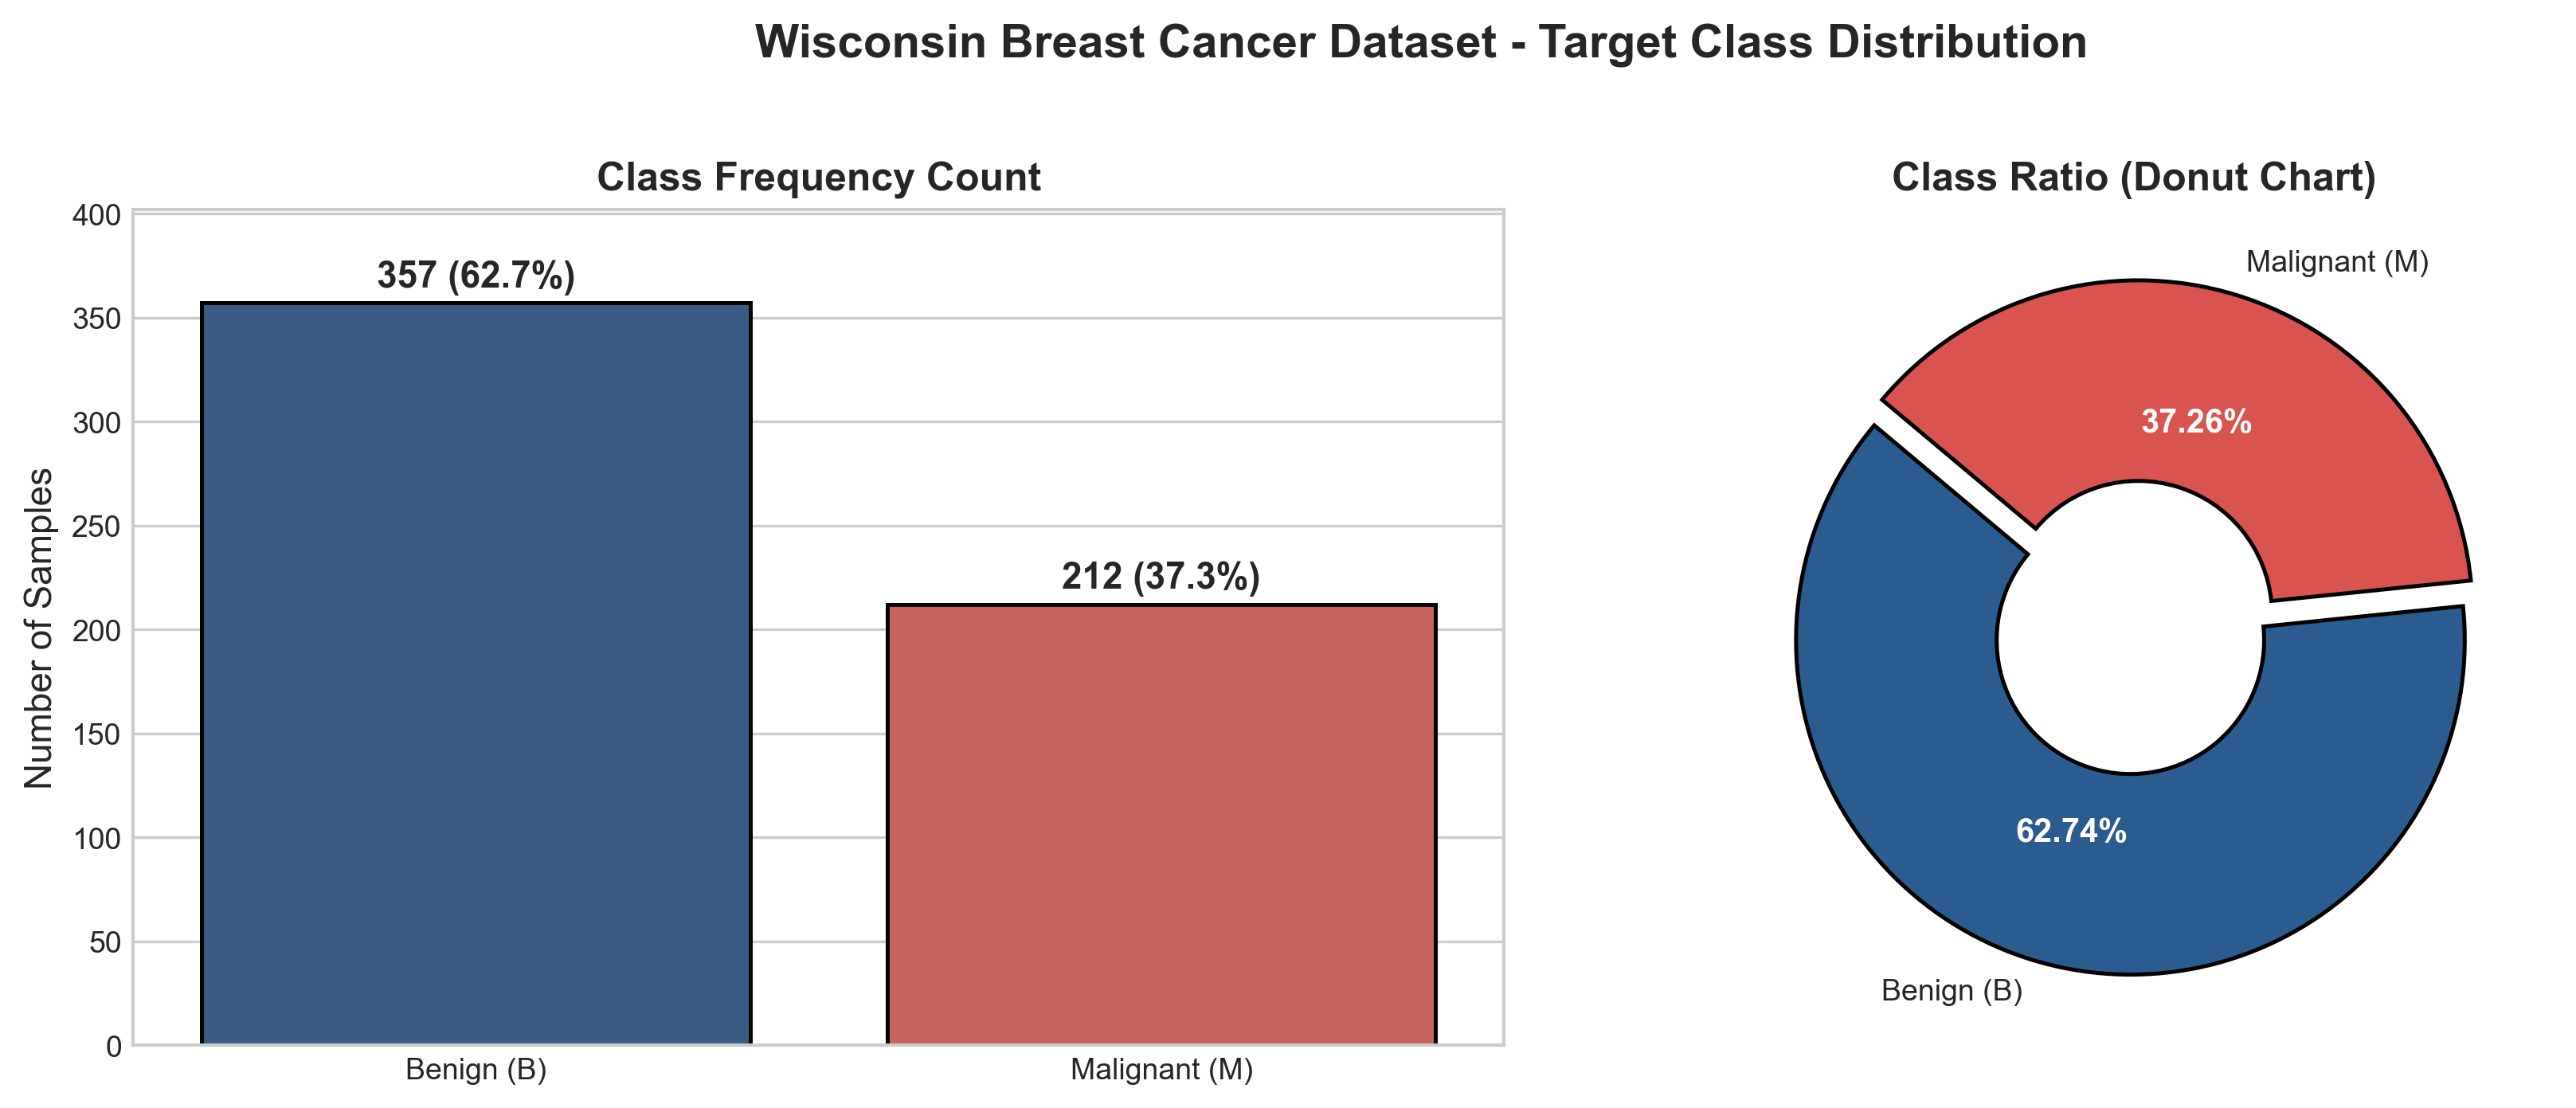
\includegraphics[width=0.9\linewidth]{eda_class_distribution.png}
\caption{Target Class Frequency and Proportion (Benign vs. Malignant)}
\label{fig:class_dist}
\end{figure}

\textbf{Inference:} The dataset exhibits a mild class imbalance: 357 cases (62.74\%) are benign and 212 cases (37.26\%) are malignant. Stratified sampling is strictly implemented across train-test partitions and cross-validation folds to preserve label proportions.

\subsection{Feature Distributions and Cytological Density}
\begin{figure}[H]
\centering
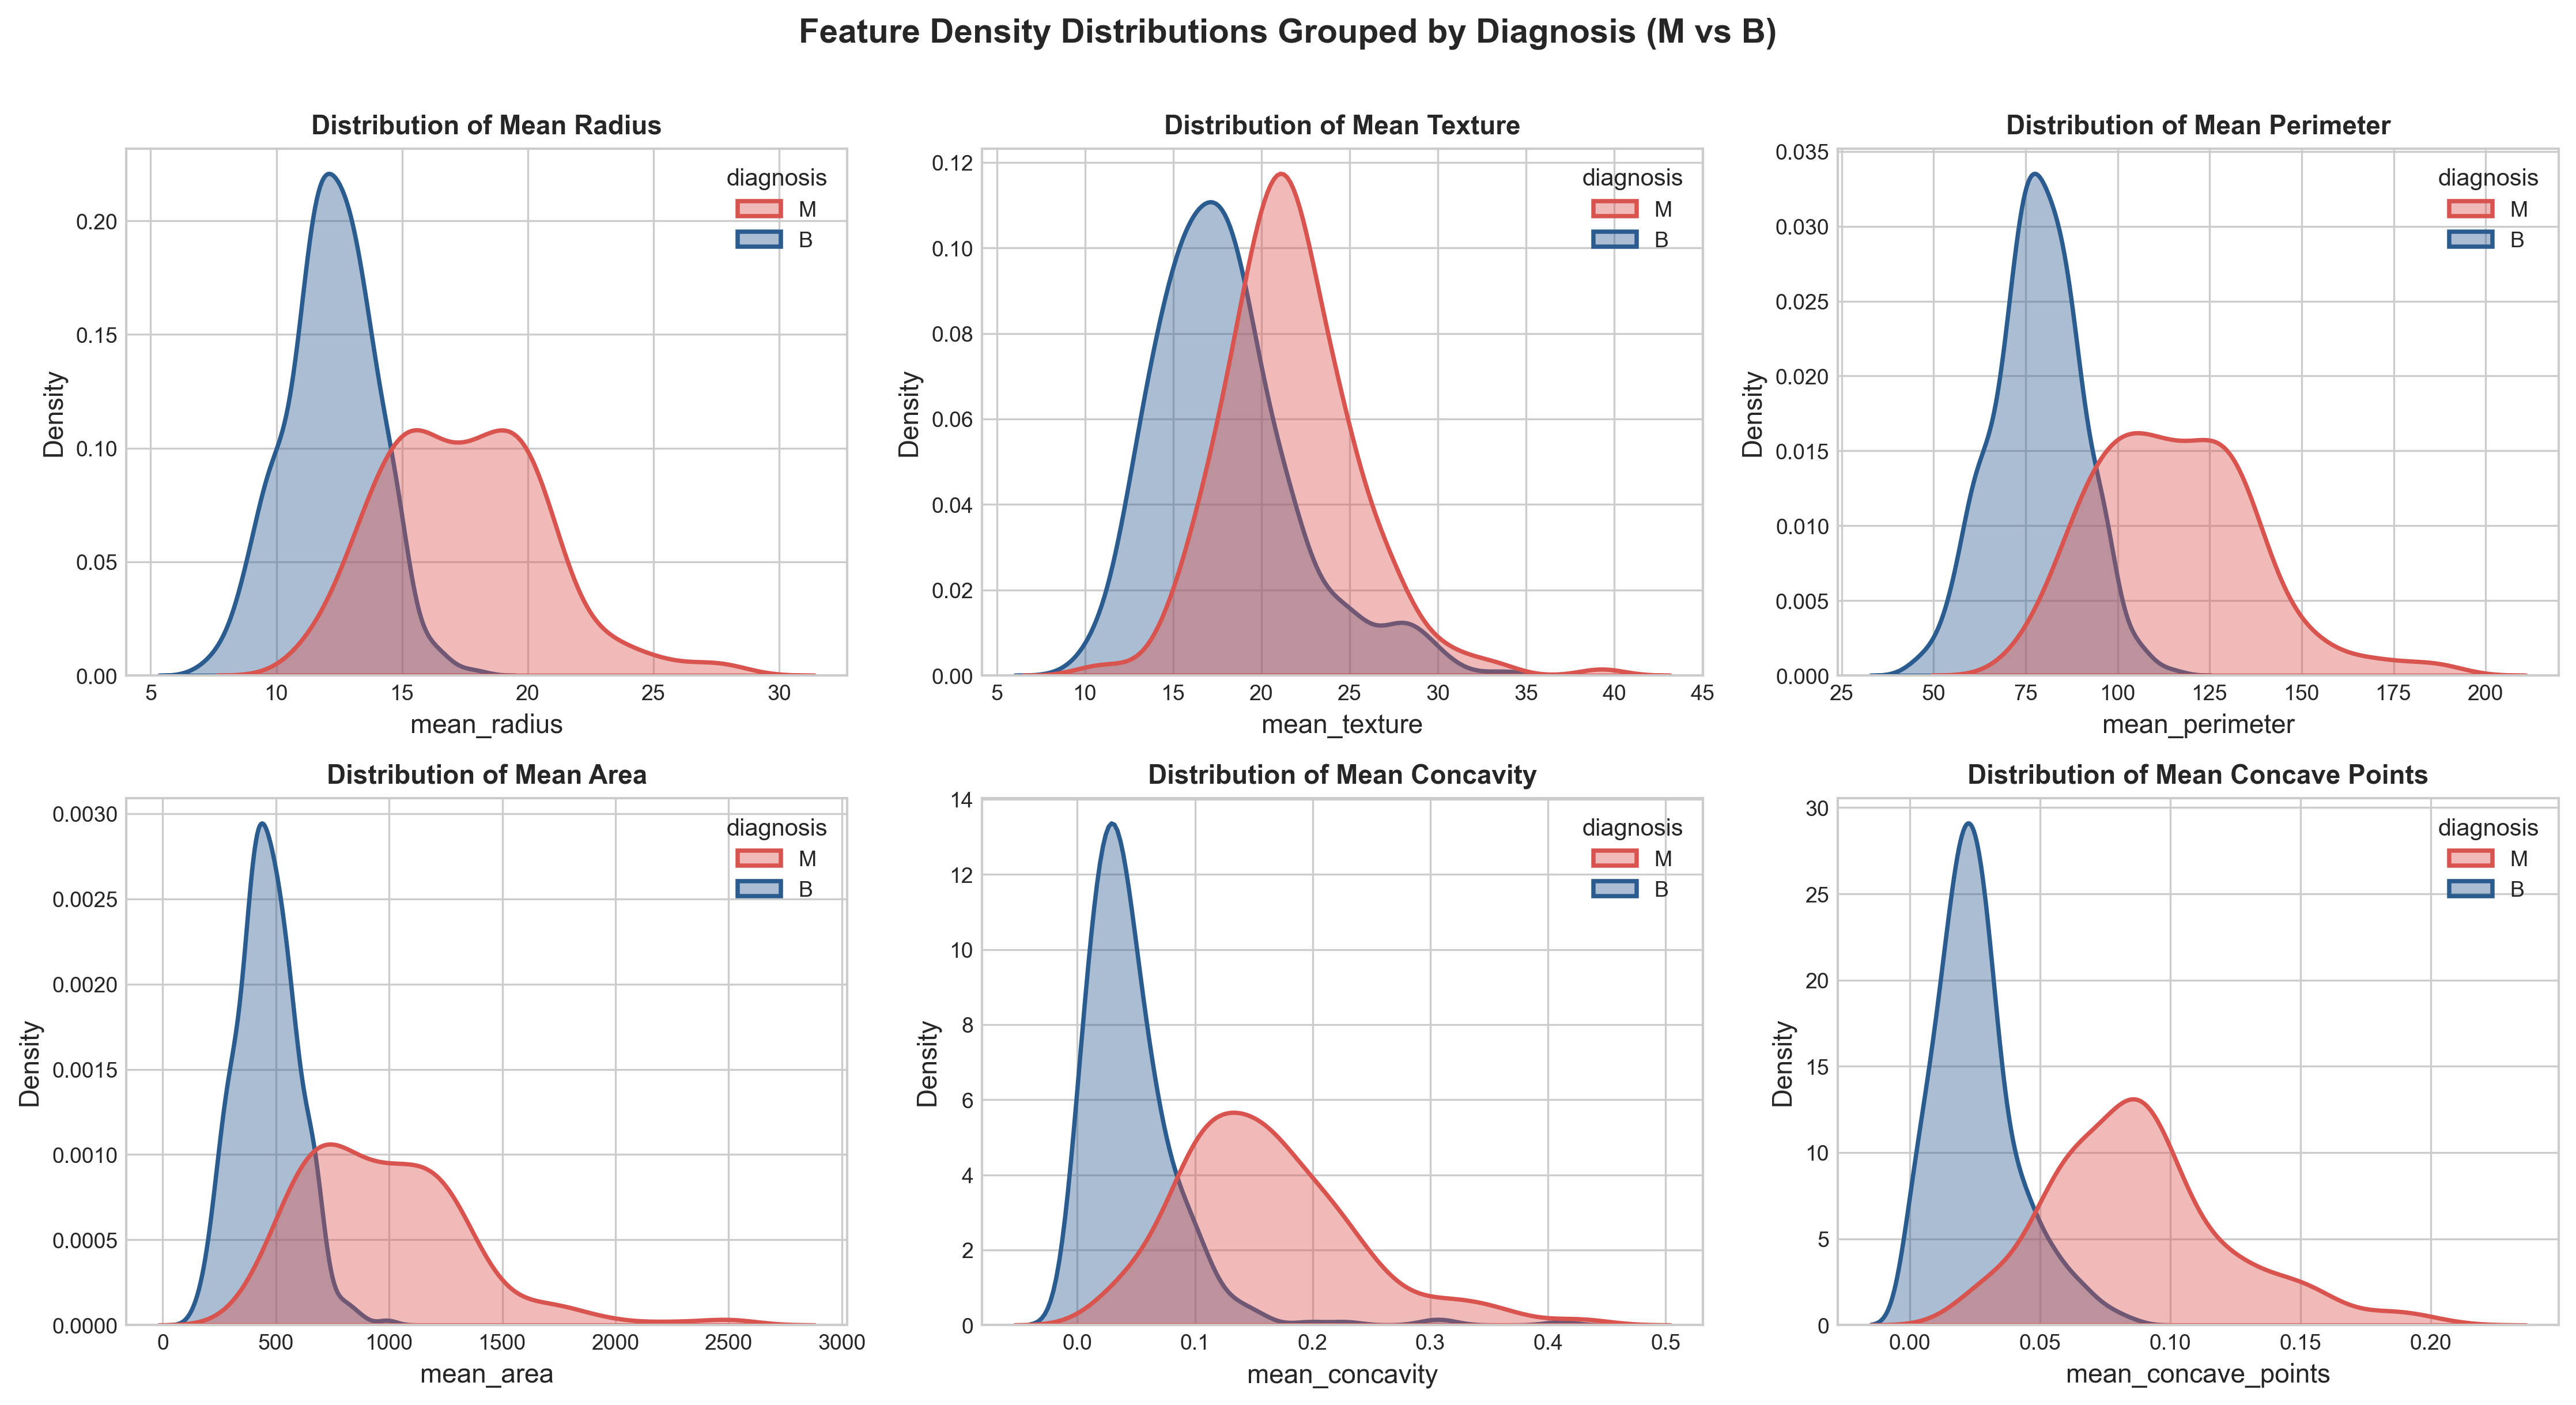
\includegraphics[width=0.95\linewidth]{eda_feature_distributions.png}
\caption{Density Distributions of Key Nuclear Morphology Features Grouped by Diagnosis}
\label{fig:feat_dist}
\end{figure}

\textbf{Inference:} Malignant nuclei systematically demonstrate significantly higher mean radius, mean perimeter, mean area, and concave point density. The pronounced bimodal separation in features such as \texttt{mean\_concave\_points} and \texttt{mean\_radius} provides strong discriminative signal for non-linear boundaries.

\subsection{Correlation Heatmap and Multicollinearity}
\begin{figure}[H]
\centering
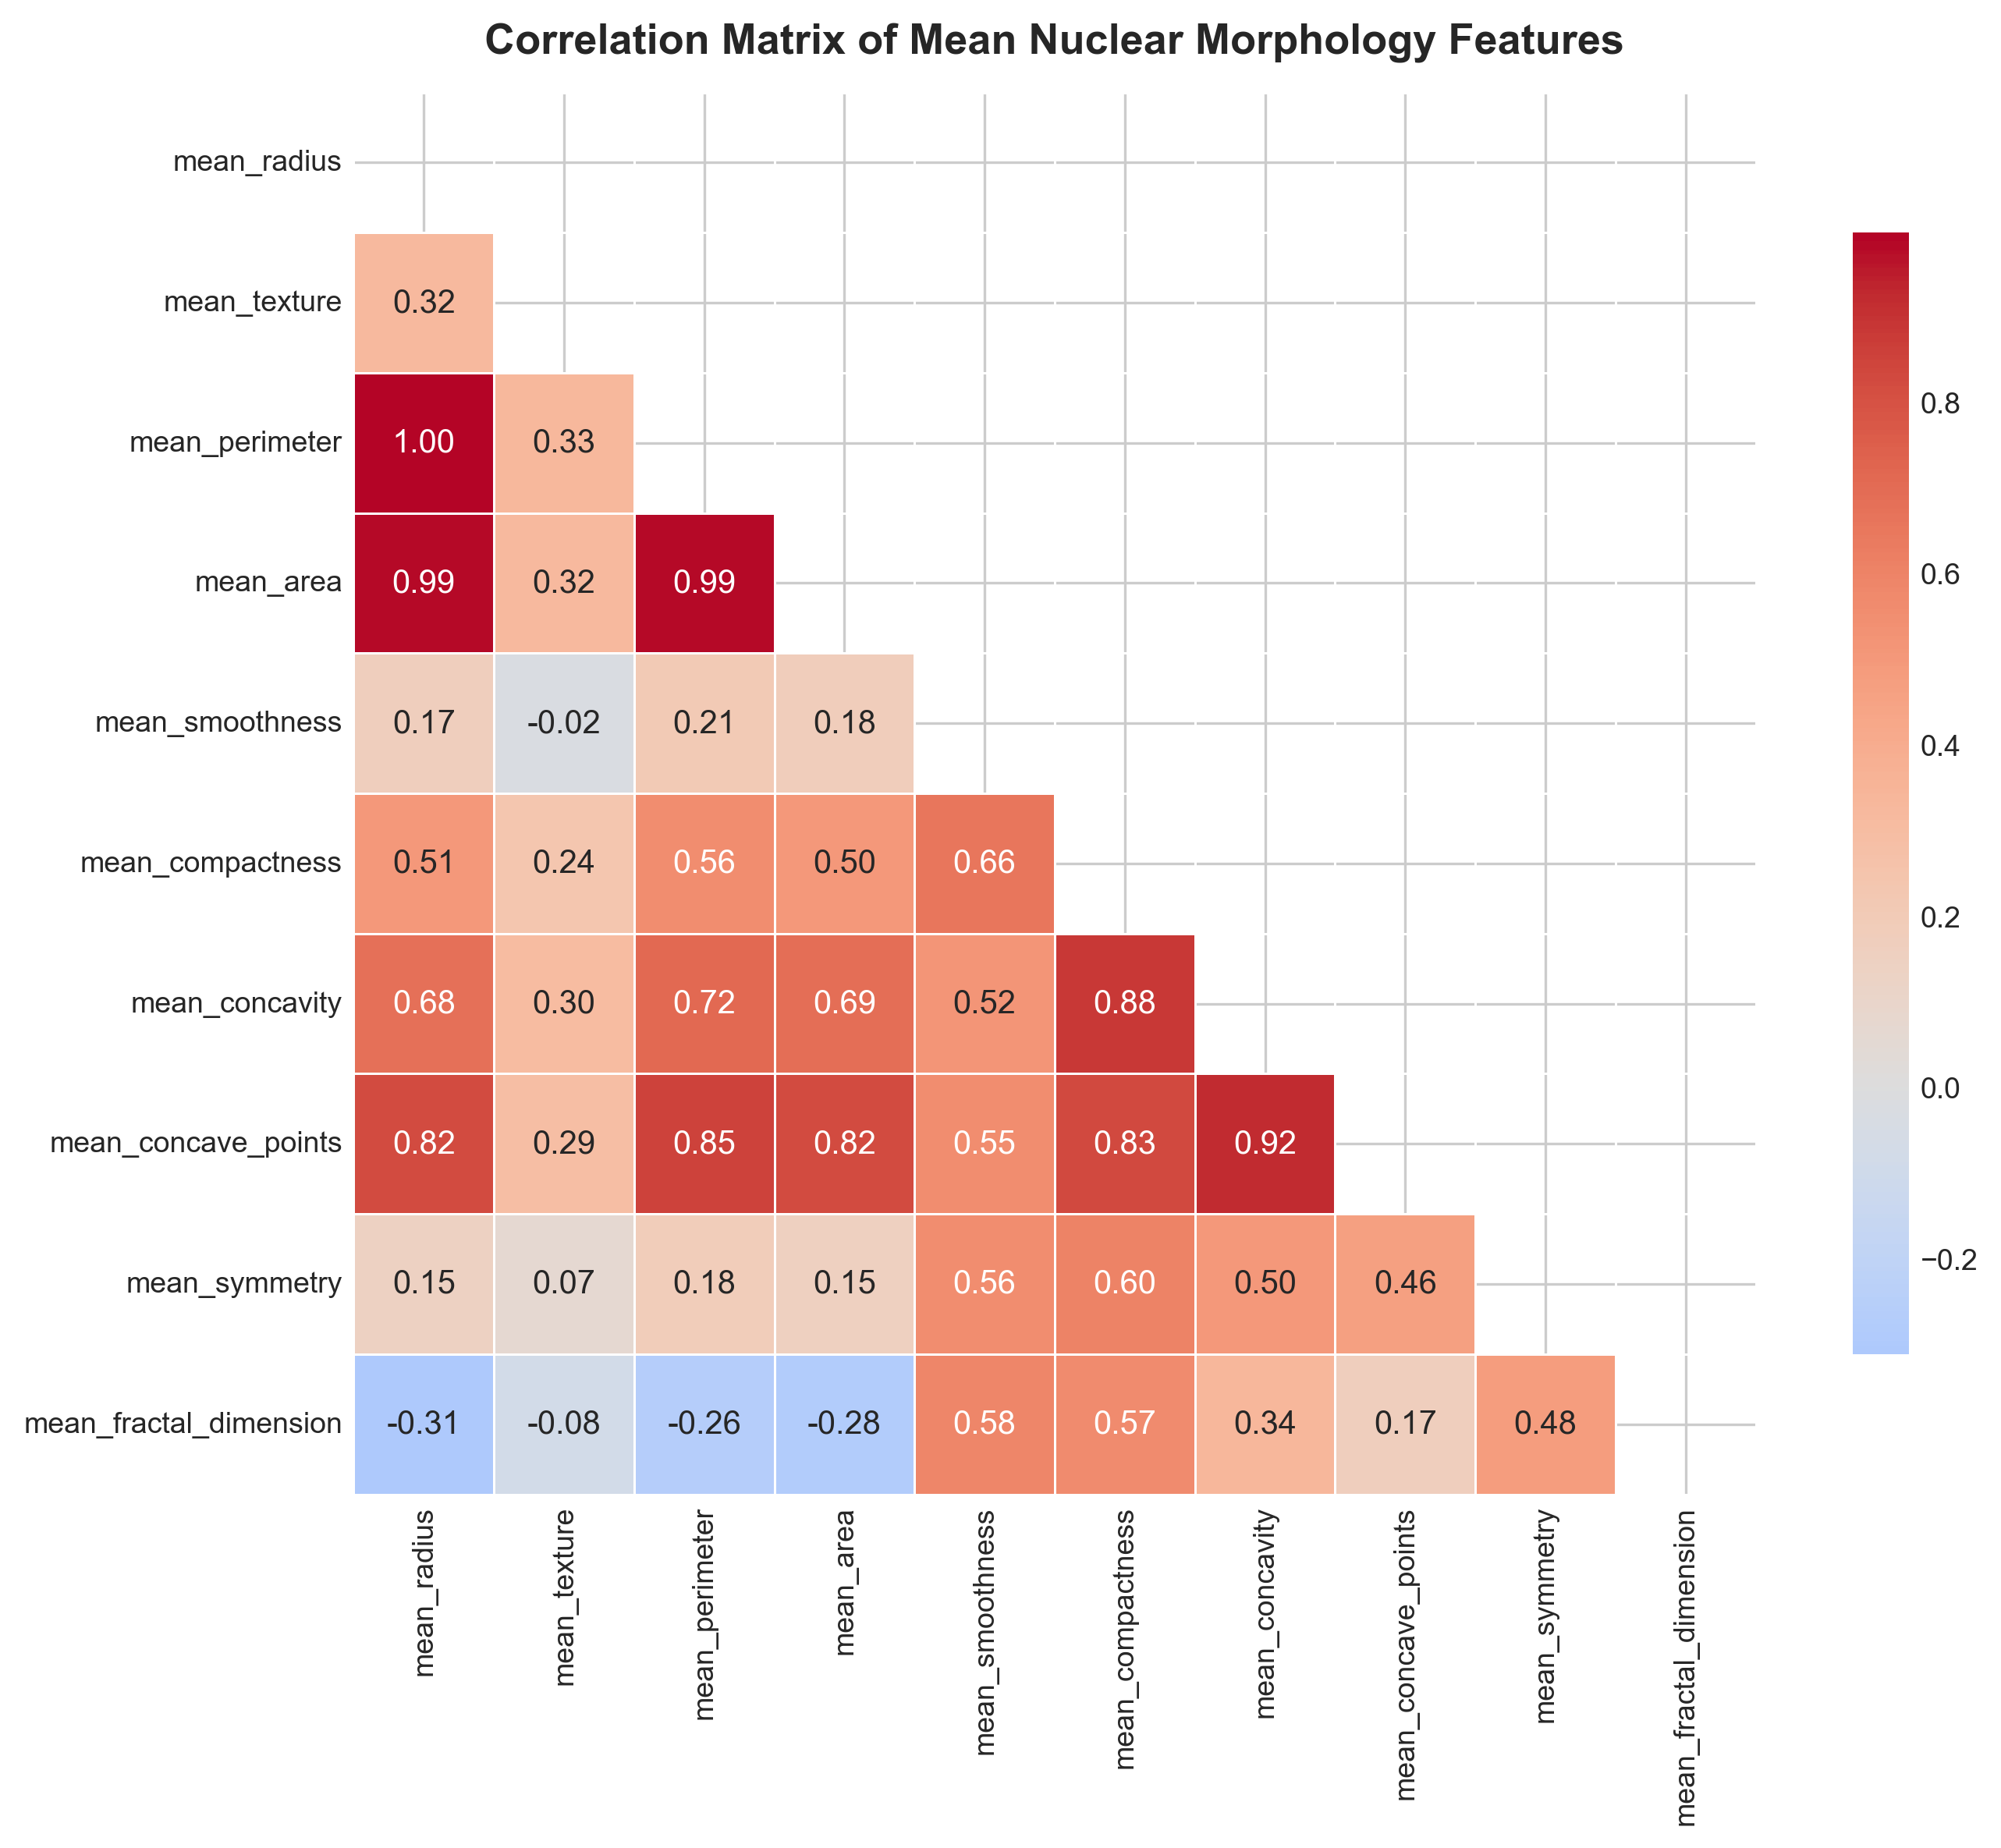
\includegraphics[width=0.75\linewidth]{eda_correlation_matrix.png}
\caption{Correlation Matrix of Mean Nuclear Morphology Descriptors}
\label{fig:corr}
\end{figure}

\textbf{Inference:} Severe multicollinearity is present among geometric size attributes (\texttt{mean\_radius}, \texttt{mean\_perimeter}, and \texttt{mean\_area} have pairwise Pearson $r > 0.98$). Tree-based ensembles naturally handle multicollinearity through recursive single-feature split selections, whereas distance-sensitive learners (SVM, Logistic Regression) benefit from feature scaling.

\subsection{Outlier Boxplots and Feature Separability}
\begin{figure}[H]
\centering
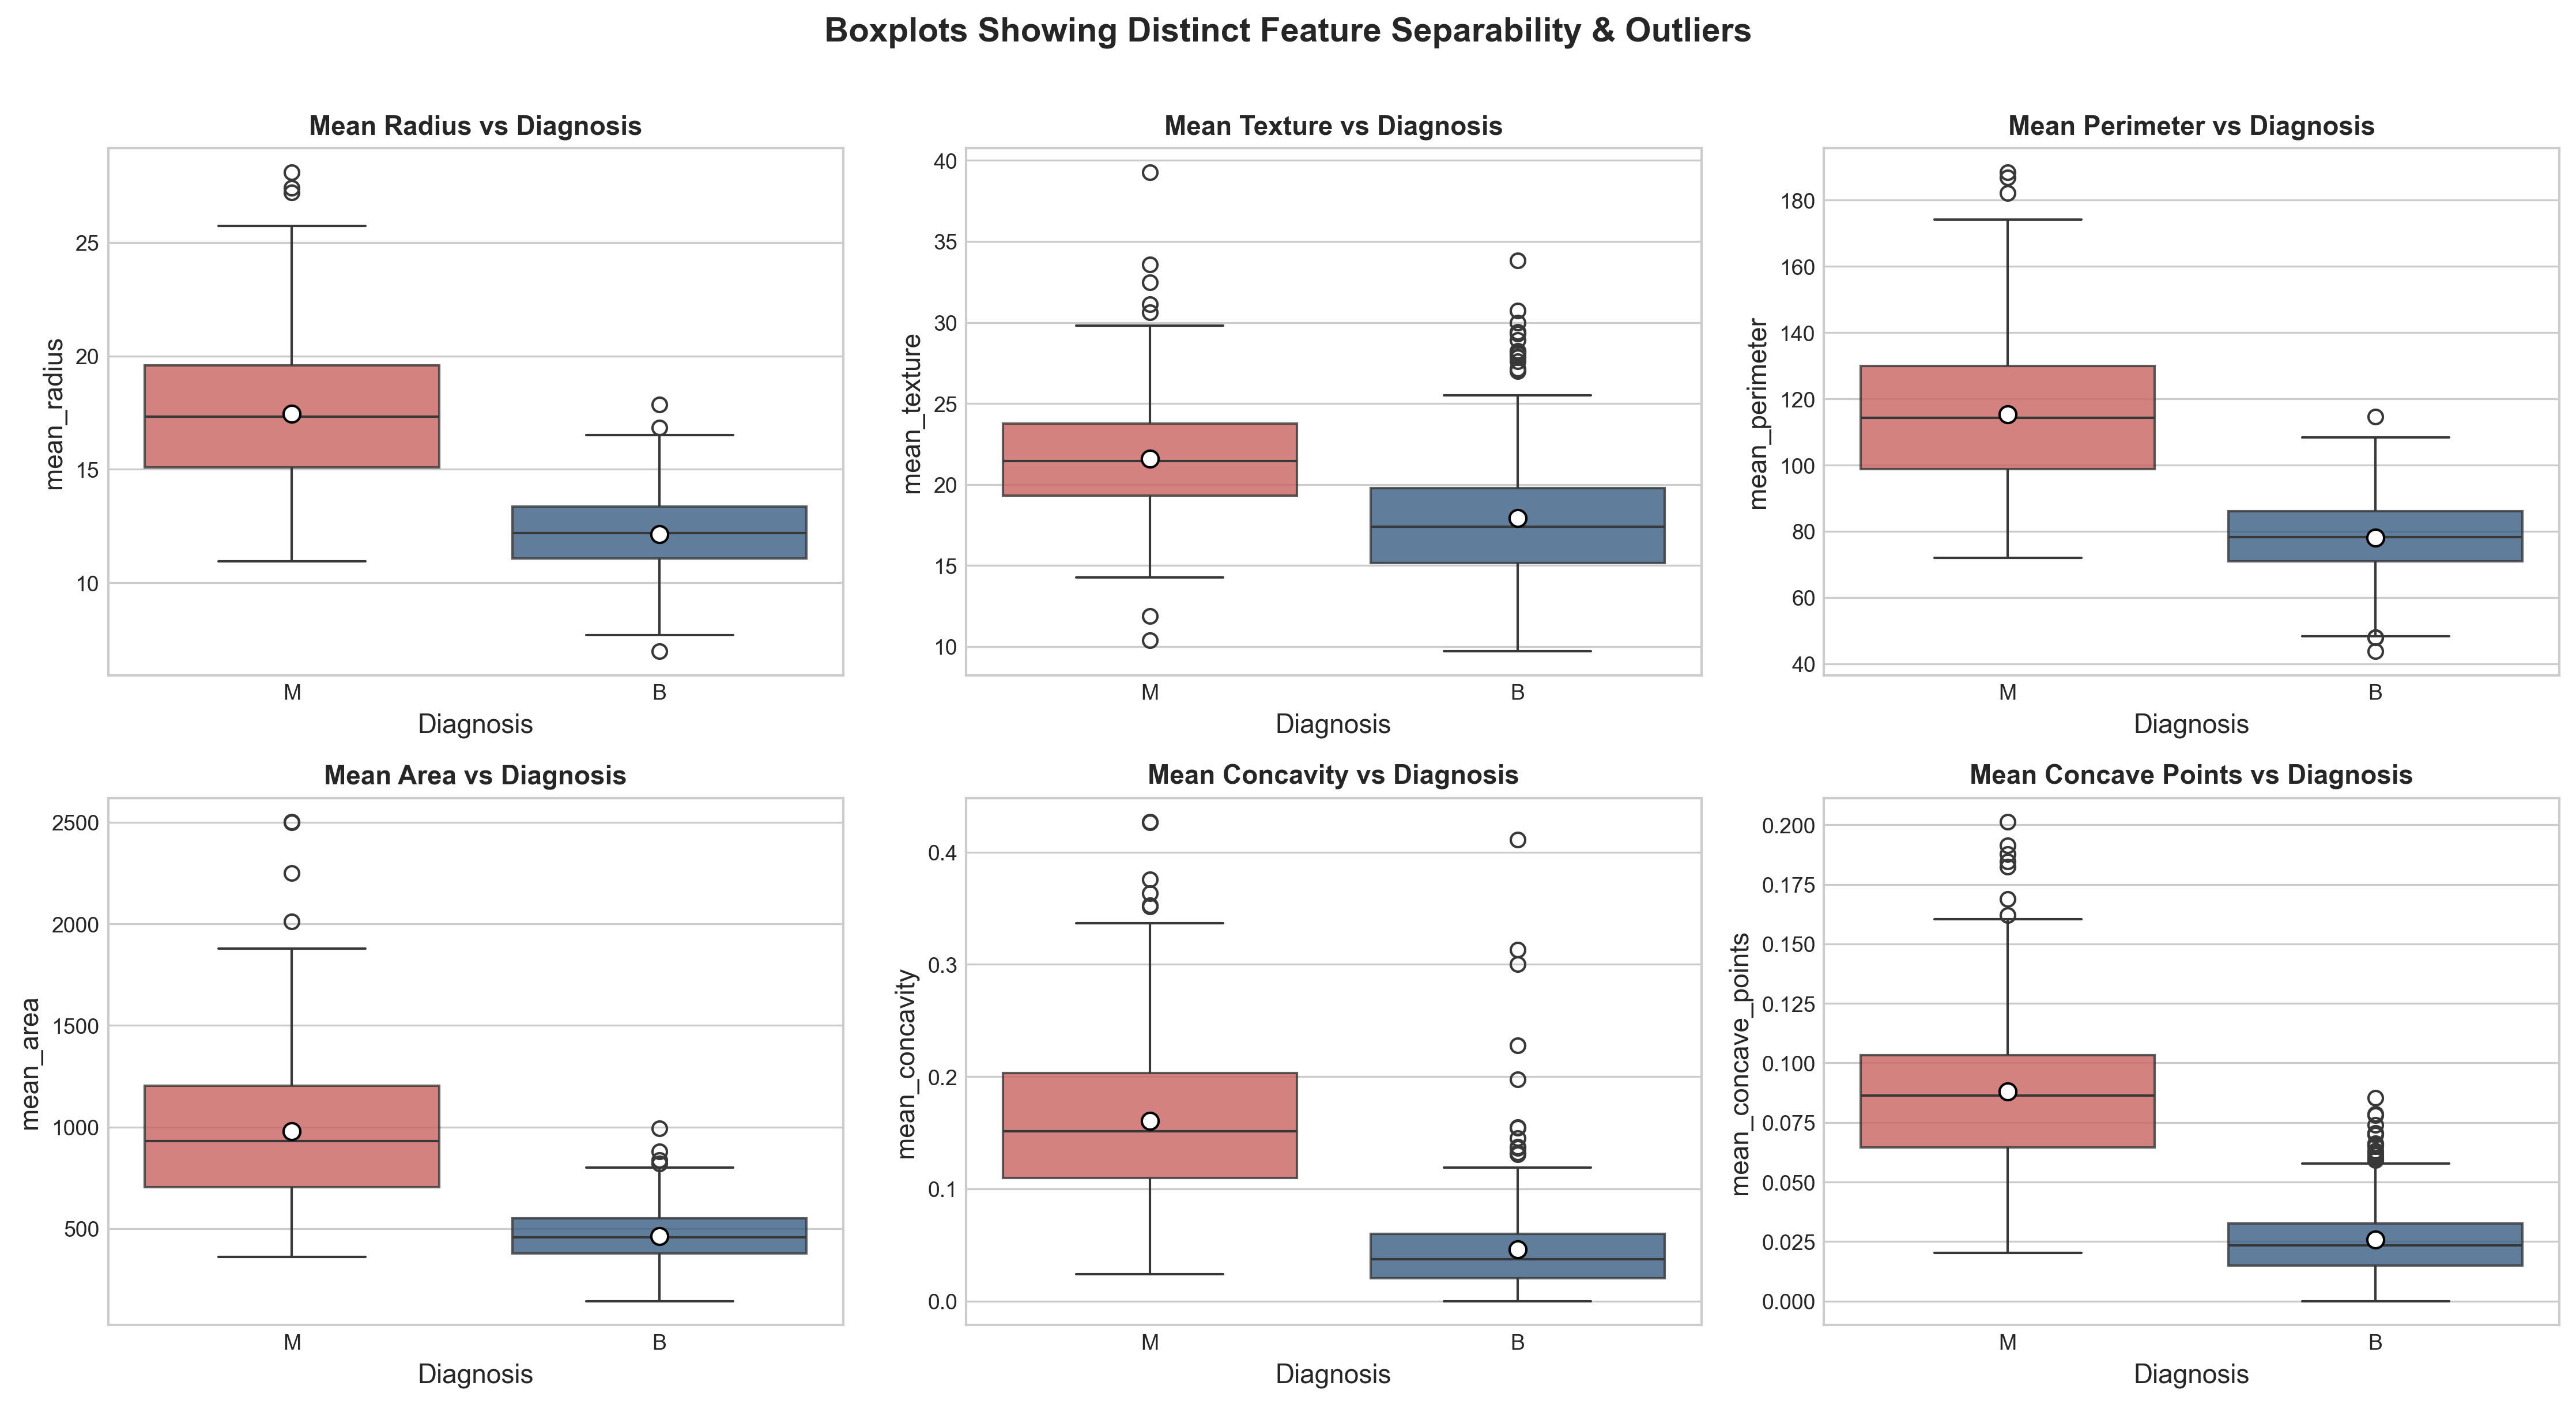
\includegraphics[width=0.95\linewidth]{eda_boxplots_outliers.png}
\caption{Boxplots Depicting Feature Separability and Outlier Densities}
\label{fig:boxplots}
\end{figure}

\textbf{Inference:} Malignant biopsies show larger variance and several high-magnitude outliers in perimeter and area metrics. Robust scaling and ensemble averaging prevent individual extreme outliers from skewing model decisions.

\subsection{2D Principal Component Projection}
\begin{figure}[H]
\centering
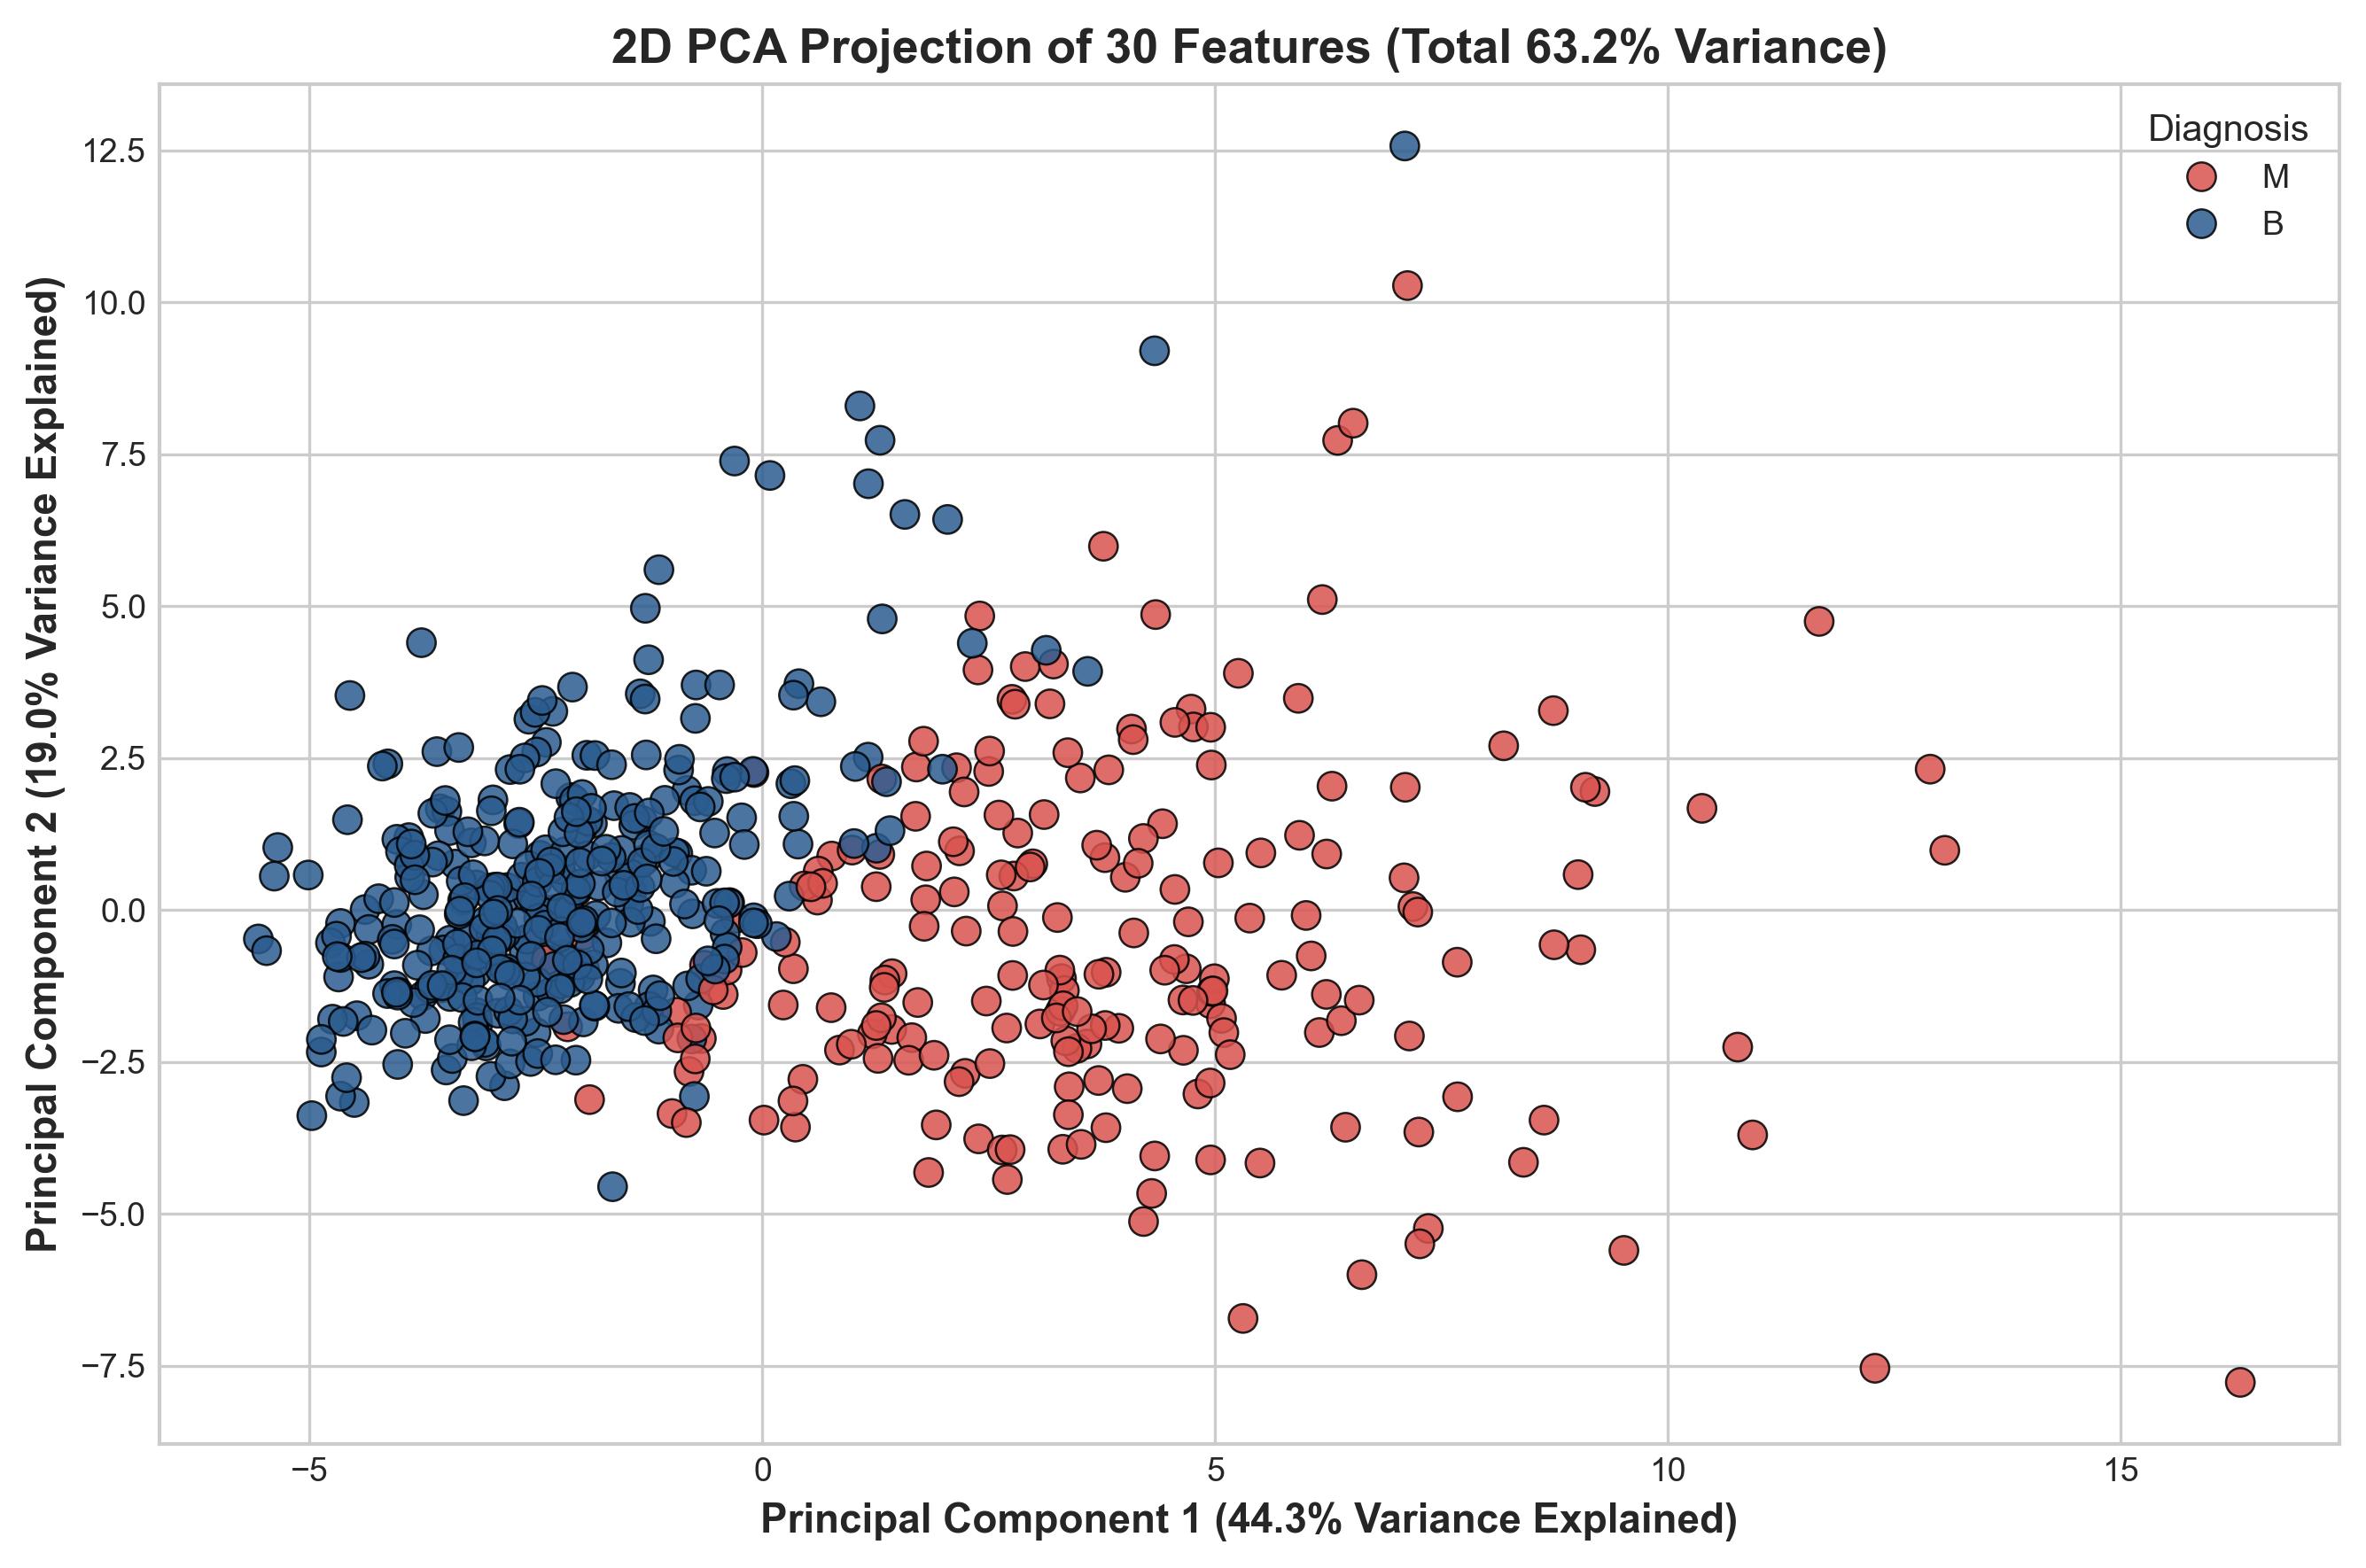
\includegraphics[width=0.75\linewidth]{eda_pca_projection.png}
\caption{Two-Dimensional PCA Projection of the 30-Dimensional Feature Space}
\label{fig:pca}
\end{figure}

\textbf{Inference:} The first two principal components capture 63.2\% of total dataset variance (PC1: 44.3\%, PC2: 19.0\%). A distinct non-linear boundary separates malignant and benign clusters, demonstrating that kernelized SVM and non-linear ensembles can achieve near-optimal decision boundaries.

\section{Methodology and Step-by-Step Implementation}
\begin{enumerate}
    \item \textbf{Data Ingestion \& Target Standardization:} The 569 WDBC biopsy records are loaded, column names formatted, missing values checked (0 found), and diagnosis mapped to binary clinical format ($1 = \text{Malignant}, 0 = \text{Benign}$).
    \item \textbf{Stratified Splitting:} An 80\% training (455 samples) and 20\% test (114 samples) partition is created with \texttt{random\_state=42} and stratified labels.
    \item \textbf{Feature Standardization:} Continuous inputs are standardized to zero mean and unit variance ($\mu=0, \sigma=1$) using \texttt{StandardScaler} fit strictly on the training partition.
    \item \textbf{5-Fold Stratified Cross-Validation:} A 5-fold cross-validation scheme evaluates hyperparameter grids for Bagging, Boosting, and Stacking.
    \item \textbf{Bagging Tuning:} Evaluates $n\_estimators \in \{10, 25, 50, 100, 200\}$ and $max\_samples \in \{0.5, 0.7, 0.8, 1.0\}$.
    \item \textbf{Boosting Tuning:} Evaluates combinations of $n\_estimators \in \{20, 50, 100, 200\}$, learning rate $\eta \in \{0.01, 0.05, 0.1, 0.2, 0.5, 1.0\}$, and tree depth for AdaBoost and Gradient Boosting.
    \item \textbf{Stacked Ensemble Construction:} Constructs out-of-fold probability blends using SVM (RBF), Gaussian Na\"ive Bayes, and Decision Tree base learners fed into Logistic Regression.
    \item \textbf{Test Benchmark \& Diagnostic Evaluation:} Evaluates all models on the held-out 114 test samples, plotting Confusion Matrices, ROC curves, Precision-Recall curves, feature importances, and runtimes.
    \item \textbf{Empirical Bias-Variance Decomposition:} Runs 50 bootstrap resamplings on the test partition to quantify bias, variance, and overall error rates.
\end{enumerate}

\section{Hyperparameter Evaluation Results}

\subsection{Bagging Hyperparameter Evaluation}
Table \ref{tab:bagging_results} documents 5-fold cross-validation performance across varying bootstrap sample fractions ($max\_samples$) and ensemble sizes ($n\_estimators$).

\begin{table}[H]
\centering
\caption{Table 1: Bagging Hyperparameter Evaluation (5-Fold Stratified CV)}
\label{tab:bagging_results}
\begin{tabular}{|c|c|c|c|}
\hline
\textbf{n\_estimators} & \textbf{max\_samples} & \textbf{Avg CV Accuracy (\%)} & \textbf{Avg CV F1 Score} \\ \hline
10 & 0.5 & 94.07 & 0.9163 \\ \hline
10 & 0.7 & 94.73 & 0.9261 \\ \hline
10 & 0.8 & 94.51 & 0.9226 \\ \hline
10 & 1.0 & 96.04 & 0.9459 \\ \hline
25 & 0.5 & 95.60 & 0.9404 \\ \hline
25 & 0.7 & 96.26 & 0.9492 \\ \hline
25 & 0.8 & 96.92 & 0.9585 \\ \hline
\textbf{25} & \textbf{1.0} & \textbf{97.14} & \textbf{0.9621} \\ \hline
50 & 0.5 & 95.82 & 0.9434 \\ \hline
50 & 0.7 & 96.04 & 0.9463 \\ \hline
50 & 0.8 & 96.92 & 0.9585 \\ \hline
50 & 1.0 & 96.48 & 0.9526 \\ \hline
100 & 0.5 & 95.82 & 0.9431 \\ \hline
100 & 0.7 & 96.26 & 0.9493 \\ \hline
100 & 0.8 & 96.48 & 0.9525 \\ \hline
100 & 1.0 & 96.48 & 0.9525 \\ \hline
200 & 0.5 & 95.82 & 0.9431 \\ \hline
200 & 0.7 & 96.26 & 0.9493 \\ \hline
200 & 0.8 & 96.70 & 0.9556 \\ \hline
200 & 1.0 & 96.70 & 0.9556 \\ \hline
\end{tabular}
\end{table}

\begin{figure}[H]
\centering
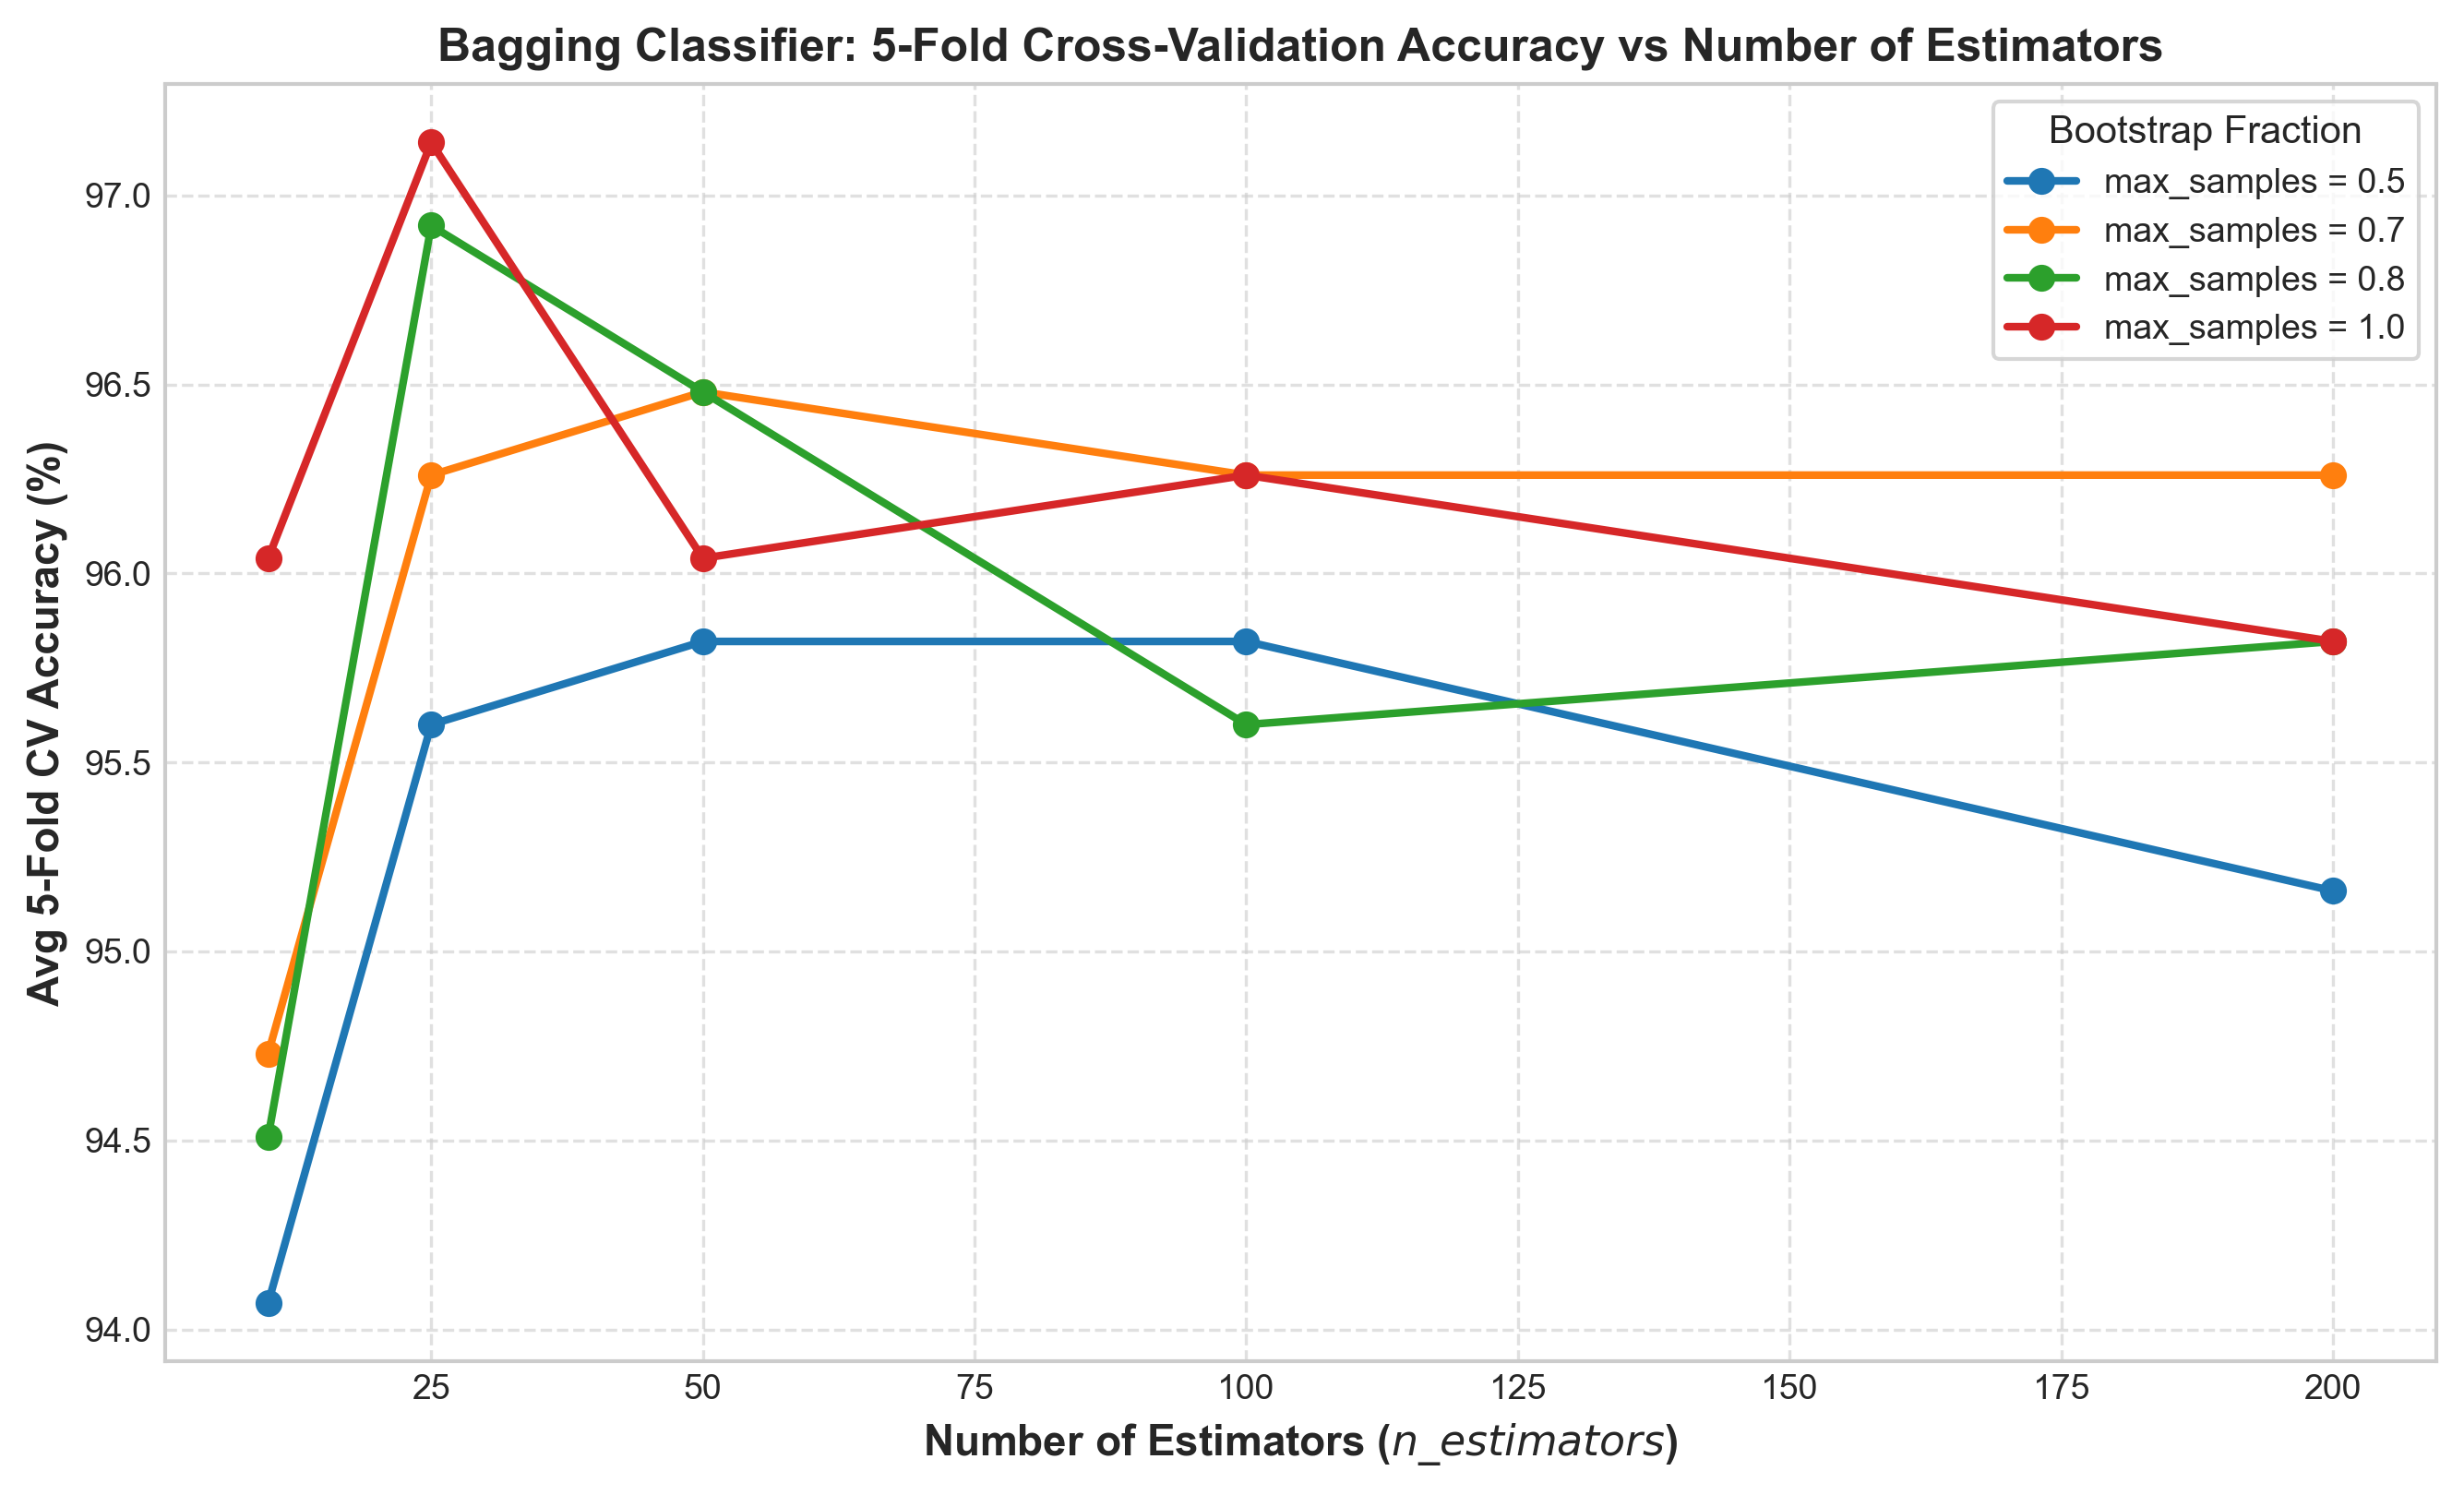
\includegraphics[width=0.75\linewidth]{bagging_hyperparameter_curve.png}
\caption{Bagging 5-Fold Cross-Validation Accuracy vs. Number of Estimators}
\label{fig:bag_curve}
\end{figure}

\textbf{Inference:} Bagging accuracy rapidly improves as ensemble size expands from 10 to 25 trees, reaching peak 5-fold CV accuracy of \textbf{97.14\%} and F1-score of \textbf{0.9621} with $max\_samples = 1.0$. Beyond 25 estimators, variance reduction saturates, confirming theoretical convergence without risk of overfitting.

\subsection{Boosting Hyperparameter Evaluation}
Table \ref{tab:boosting_results} presents cross-validation performance across boosting algorithms, learning rates ($\eta$), and tree depths.

\begin{table}[H]
\centering
\caption{Table 2: Boosting Hyperparameter Evaluation (5-Fold Stratified CV)}
\label{tab:boosting_results}
\begin{tabular}{|l|c|c|c|c|c|}
\hline
\textbf{Algorithm} & \textbf{n\_estimators} & \textbf{learning\_rate} & \textbf{max\_depth} & \textbf{Avg CV Acc (\%)} & \textbf{Avg CV F1} \\ \hline
Gradient Boosting & 20 & 0.01 & 2 & 92.75 & 0.8938 \\ \hline
Gradient Boosting & 20 & 0.10 & 2 & 95.82 & 0.9435 \\ \hline
Gradient Boosting & 50 & 0.01 & 2 & 93.63 & 0.9084 \\ \hline
Gradient Boosting & 50 & 0.05 & 3 & 95.82 & 0.9432 \\ \hline
Gradient Boosting & 50 & 0.10 & 3 & 96.26 & 0.9493 \\ \hline
Gradient Boosting & 100 & 0.01 & 3 & 94.51 & 0.9221 \\ \hline
Gradient Boosting & 100 & 0.05 & 3 & 96.04 & 0.9463 \\ \hline
Gradient Boosting & 100 & 0.10 & 3 & 96.48 & 0.9525 \\ \hline
Gradient Boosting & 100 & 0.20 & 3 & 96.92 & 0.9585 \\ \hline
Gradient Boosting & 200 & 0.05 & 3 & 96.48 & 0.9525 \\ \hline
Gradient Boosting & 200 & 0.10 & 3 & 96.70 & 0.9556 \\ \hline
\textbf{Gradient Boosting} & \textbf{200} & \textbf{0.20} & \textbf{2} & \textbf{97.36} & \textbf{0.9647} \\ \hline
AdaBoost & 50 & 0.10 & 1 & 95.60 & 0.9398 \\ \hline
AdaBoost & 50 & 0.50 & 1 & 96.48 & 0.9525 \\ \hline
AdaBoost & 50 & 1.00 & 1 & 96.70 & 0.9559 \\ \hline
AdaBoost & 100 & 0.10 & 1 & 95.82 & 0.9432 \\ \hline
AdaBoost & 100 & 0.50 & 1 & 96.70 & 0.9556 \\ \hline
AdaBoost & 100 & 1.00 & 1 & 96.48 & 0.9526 \\ \hline
\textbf{AdaBoost} & \textbf{200} & \textbf{0.50} & \textbf{1} & \textbf{97.14} & \textbf{0.9618} \\ \hline
AdaBoost & 200 & 1.00 & 1 & 96.48 & 0.9529 \\ \hline
\end{tabular}
\end{table}

\begin{figure}[H]
\centering
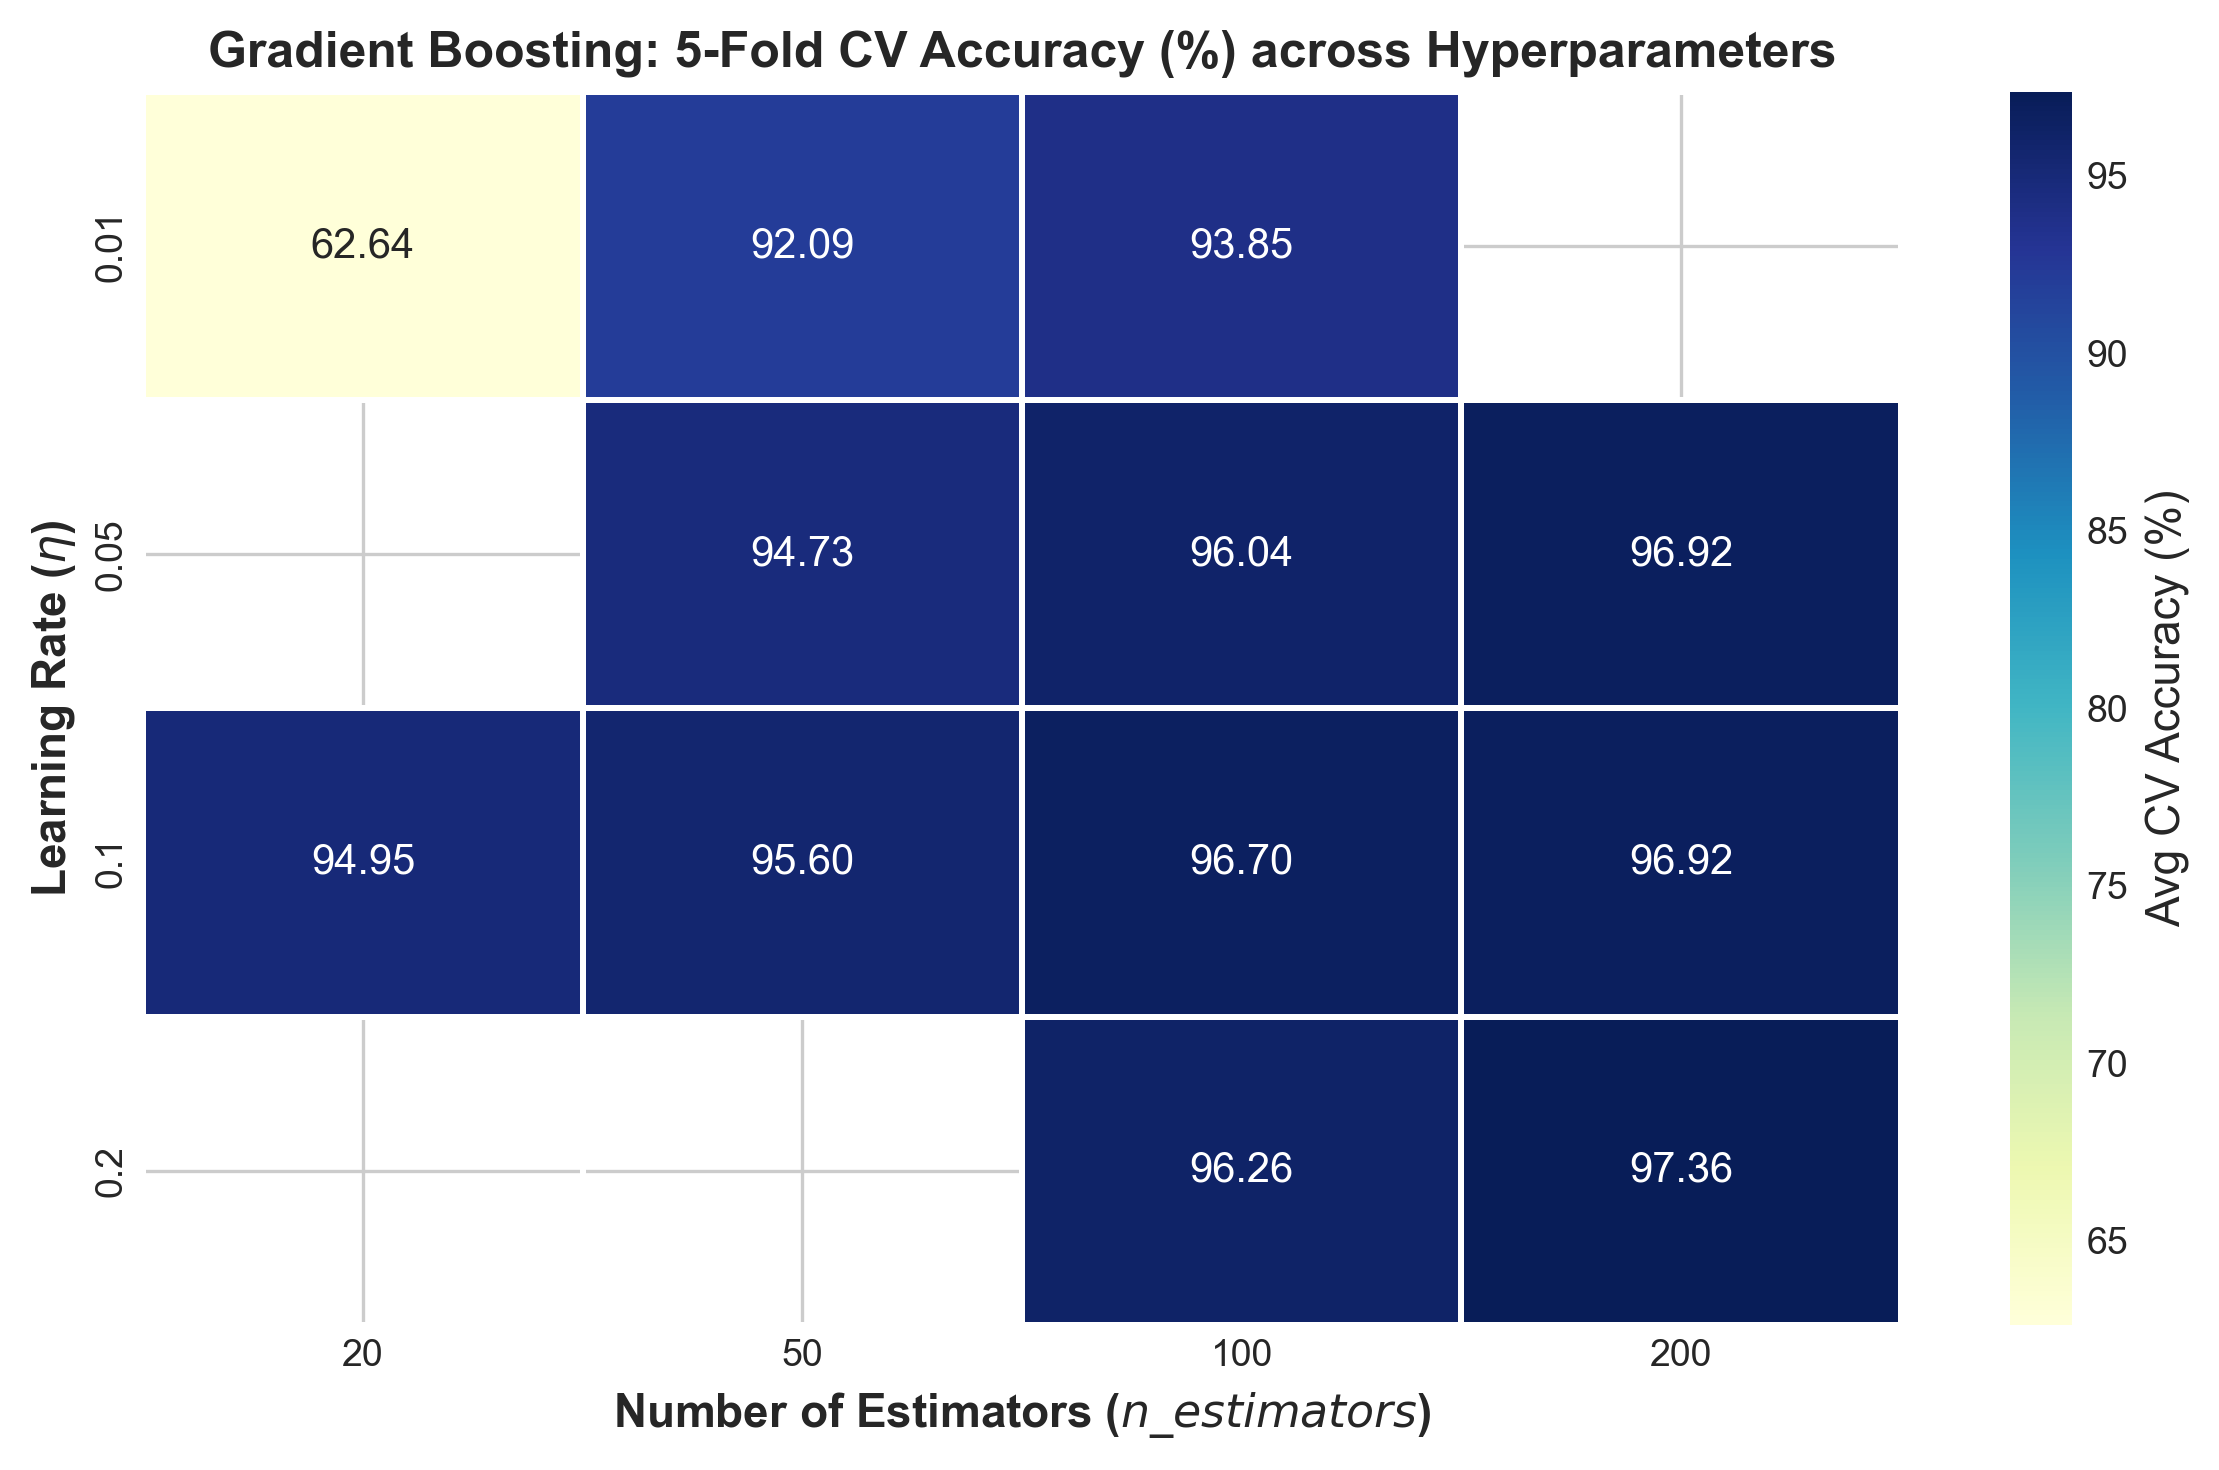
\includegraphics[width=0.65\linewidth]{boosting_hyperparameter_heatmap.png}
\caption{Gradient Boosting 5-Fold Cross-Validation Accuracy Heatmap}
\label{fig:boost_heatmap}
\end{figure}

\textbf{Inference:} Gradient Boosting achieves maximum cross-validation accuracy of \textbf{97.36\%} with shallow tree depth ($max\_depth = 2$), 200 estimators, and $\eta = 0.20$. Shallow trees constrain base learner variance, allowing additive boosting iterations to progressively minimize residual loss.

\subsection{Stacked Ensemble Evaluation}
Table \ref{tab:stacking_results} reports 5-fold cross-validation performance across base model combinations and meta-learner choices.

\begin{table}[H]
\centering
\caption{Table 3: Stacked Ensemble Evaluation (5-Fold Stratified CV)}
\label{tab:stacking_results}
\begin{tabular}{|p{6.5cm}|p{3.5cm}|c|c|}
\hline
\textbf{Base Models} & \textbf{Meta Learner} & \textbf{Avg CV Acc (\%)} & \textbf{Avg CV F1} \\ \hline
\textbf{SVM, Na\"ive Bayes, Decision Tree} & \textbf{Logistic Regression} & \textbf{96.48} & \textbf{0.9521} \\ \hline
SVM, Na\"ive Bayes & Logistic Regression & 96.48 & 0.9521 \\ \hline
\textbf{SVM, Decision Tree} & \textbf{Logistic Regression} & \textbf{96.70} & \textbf{0.9550} \\ \hline
Na\"ive Bayes, Decision Tree & Logistic Regression & 95.60 & 0.9406 \\ \hline
SVM, Na\"ive Bayes, Decision Tree & Decision Tree & 94.73 & 0.9298 \\ \hline
SVM, Na\"ive Bayes, Decision Tree & Random Forest & 95.82 & 0.9442 \\ \hline
\end{tabular}
\end{table}

\begin{figure}[H]
\centering
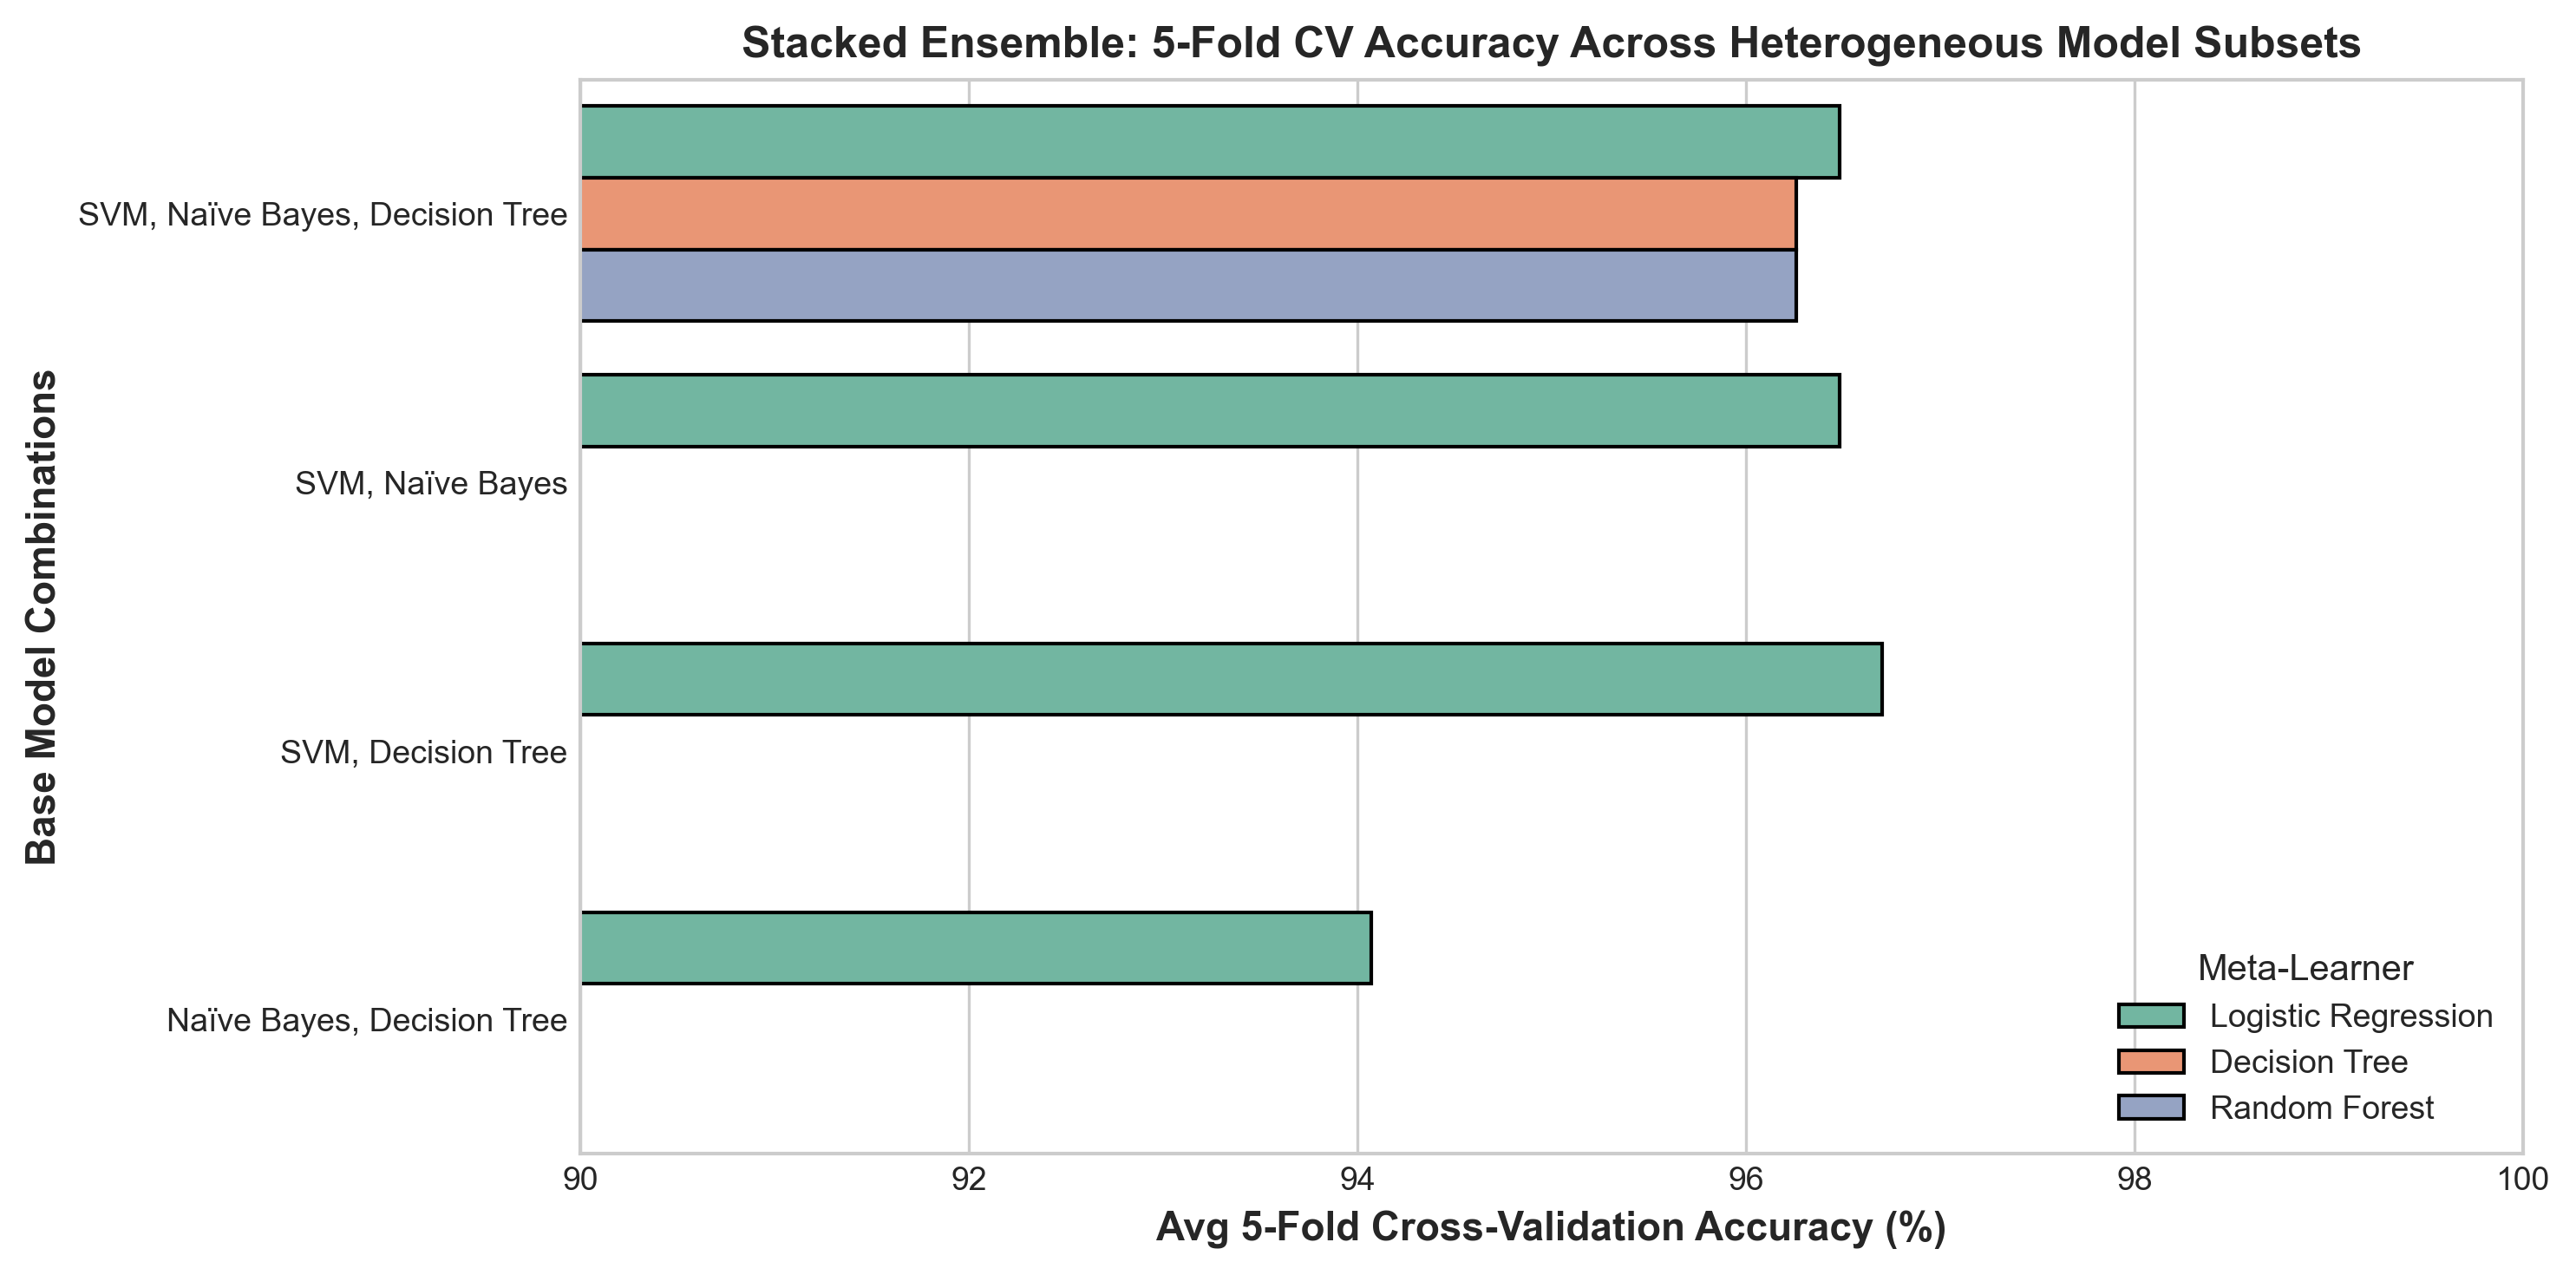
\includegraphics[width=0.75\linewidth]{stacked_ensemble_comparison.png}
\caption{Stacked Ensemble 5-Fold Cross-Validation Accuracy Across Model Subsets}
\label{fig:stack_comp}
\end{figure}

\textbf{Inference:} Logistic Regression acts as a superior meta-learner compared to tree-based meta-models, as it assigns smooth, calibrated linear blending weights over out-of-fold probability outputs without overfitting. Combining SVM with Decision Trees yields \textbf{96.70\%} CV accuracy.

\section{Performance Comparison of Ensemble Models}
Table \ref{tab:performance_comparison} provides a comprehensive benchmark of individual baseline classifiers against tuned Bagging, Boosting, and Stacked Ensemble models evaluated on the held-out 20\% test dataset (114 biopsy samples).

\begin{table}[H]
\centering
\caption{Table 4: Performance Comparison of Ensemble Models on Test Set}
\label{tab:performance_comparison}
\begin{tabular}{|l|c|c|c|c|c|}
\hline
\textbf{Model} & \textbf{Accuracy (\%)} & \textbf{Precision} & \textbf{Recall} & \textbf{F1 Score} & \textbf{ROC-AUC} \\ \hline
Baseline: Single Decision Tree & 91.23 & 0.9444 & 0.8095 & 0.8718 & 0.8770 \\ \hline
Baseline: Support Vector Machine & 97.37 & 1.0000 & 0.9286 & 0.9630 & 0.9947 \\ \hline
Baseline: Gaussian Na\"ive Bayes & 92.11 & 0.9231 & 0.8571 & 0.8889 & 0.9891 \\ \hline
\textbf{Bagging (Decision Tree)} & \textbf{97.37} & \textbf{1.0000} & \textbf{0.9286} & \textbf{0.9630} & \textbf{0.9888} \\ \hline
\textbf{AdaBoost Classifier} & \textbf{97.37} & \textbf{1.0000} & \textbf{0.9286} & \textbf{0.9630} & \textbf{0.9861} \\ \hline
\textbf{Gradient Boosting} & \textbf{96.49} & \textbf{1.0000} & \textbf{0.9048} & \textbf{0.9500} & \textbf{0.9940} \\ \hline
\textbf{Stacked Ensemble} & \textbf{96.49} & \textbf{1.0000} & \textbf{0.9048} & \textbf{0.9500} & \textbf{0.9937} \\ \hline
\end{tabular}
\end{table}

\begin{figure}[H]
\centering
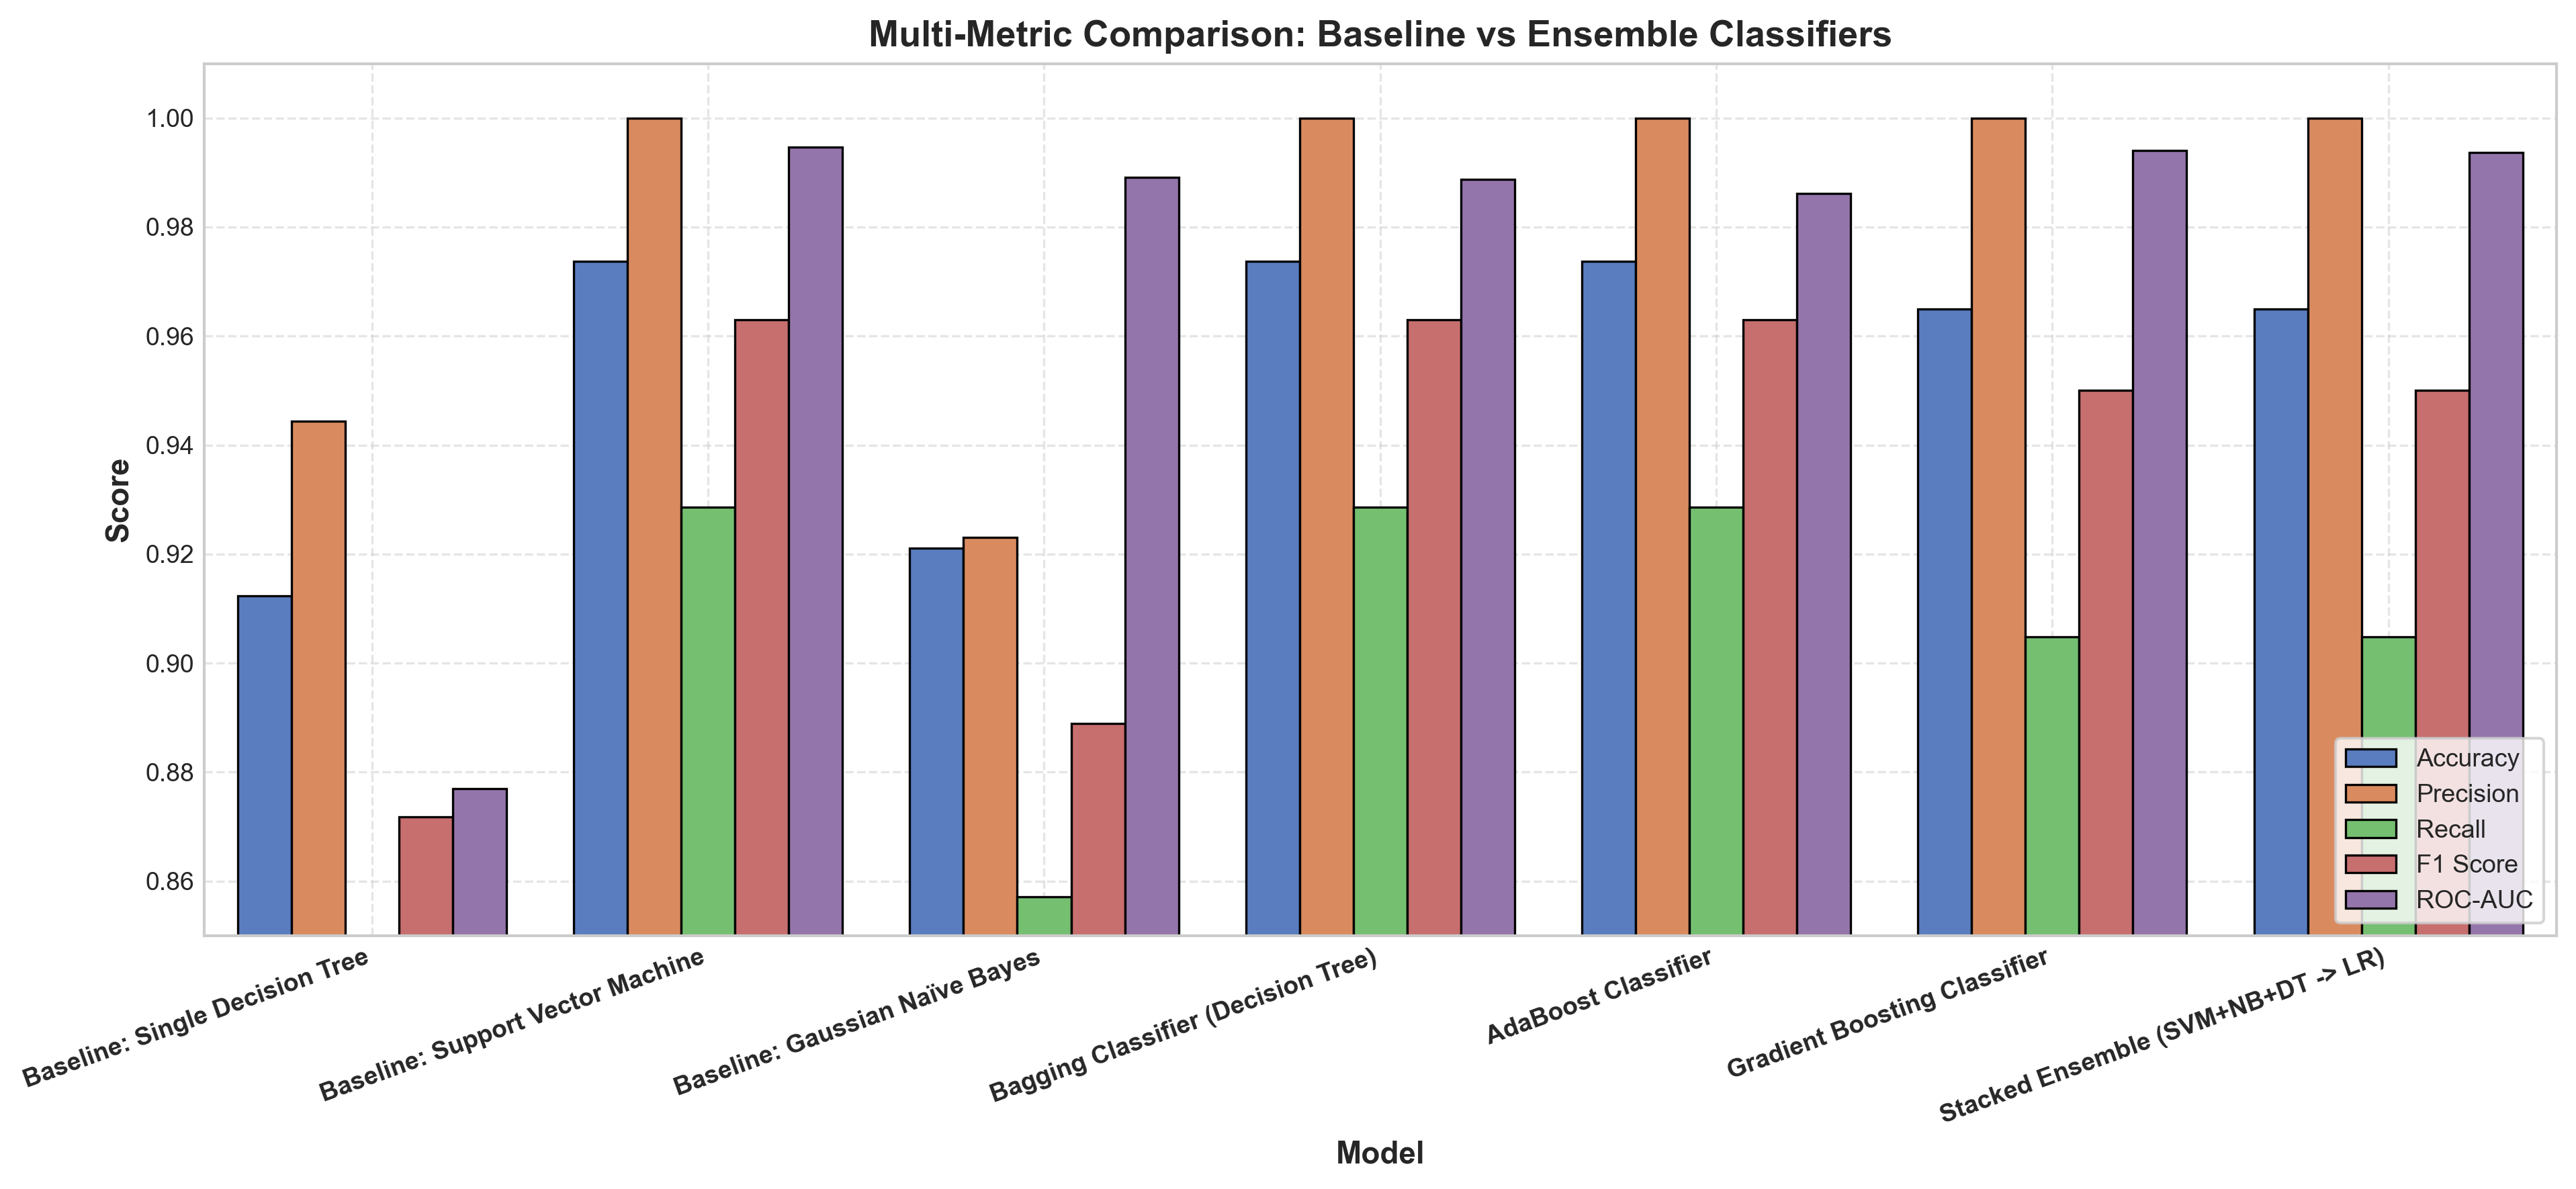
\includegraphics[width=0.95\linewidth]{model_metrics_bar_comparison.png}
\caption{Comparative Performance Across Evaluation Metrics}
\label{fig:metrics_bar}
\end{figure}

\section{Evaluation Metrics and Diagnostic Visualizations}

\subsection{Confusion Matrices}
\begin{figure}[H]
\centering
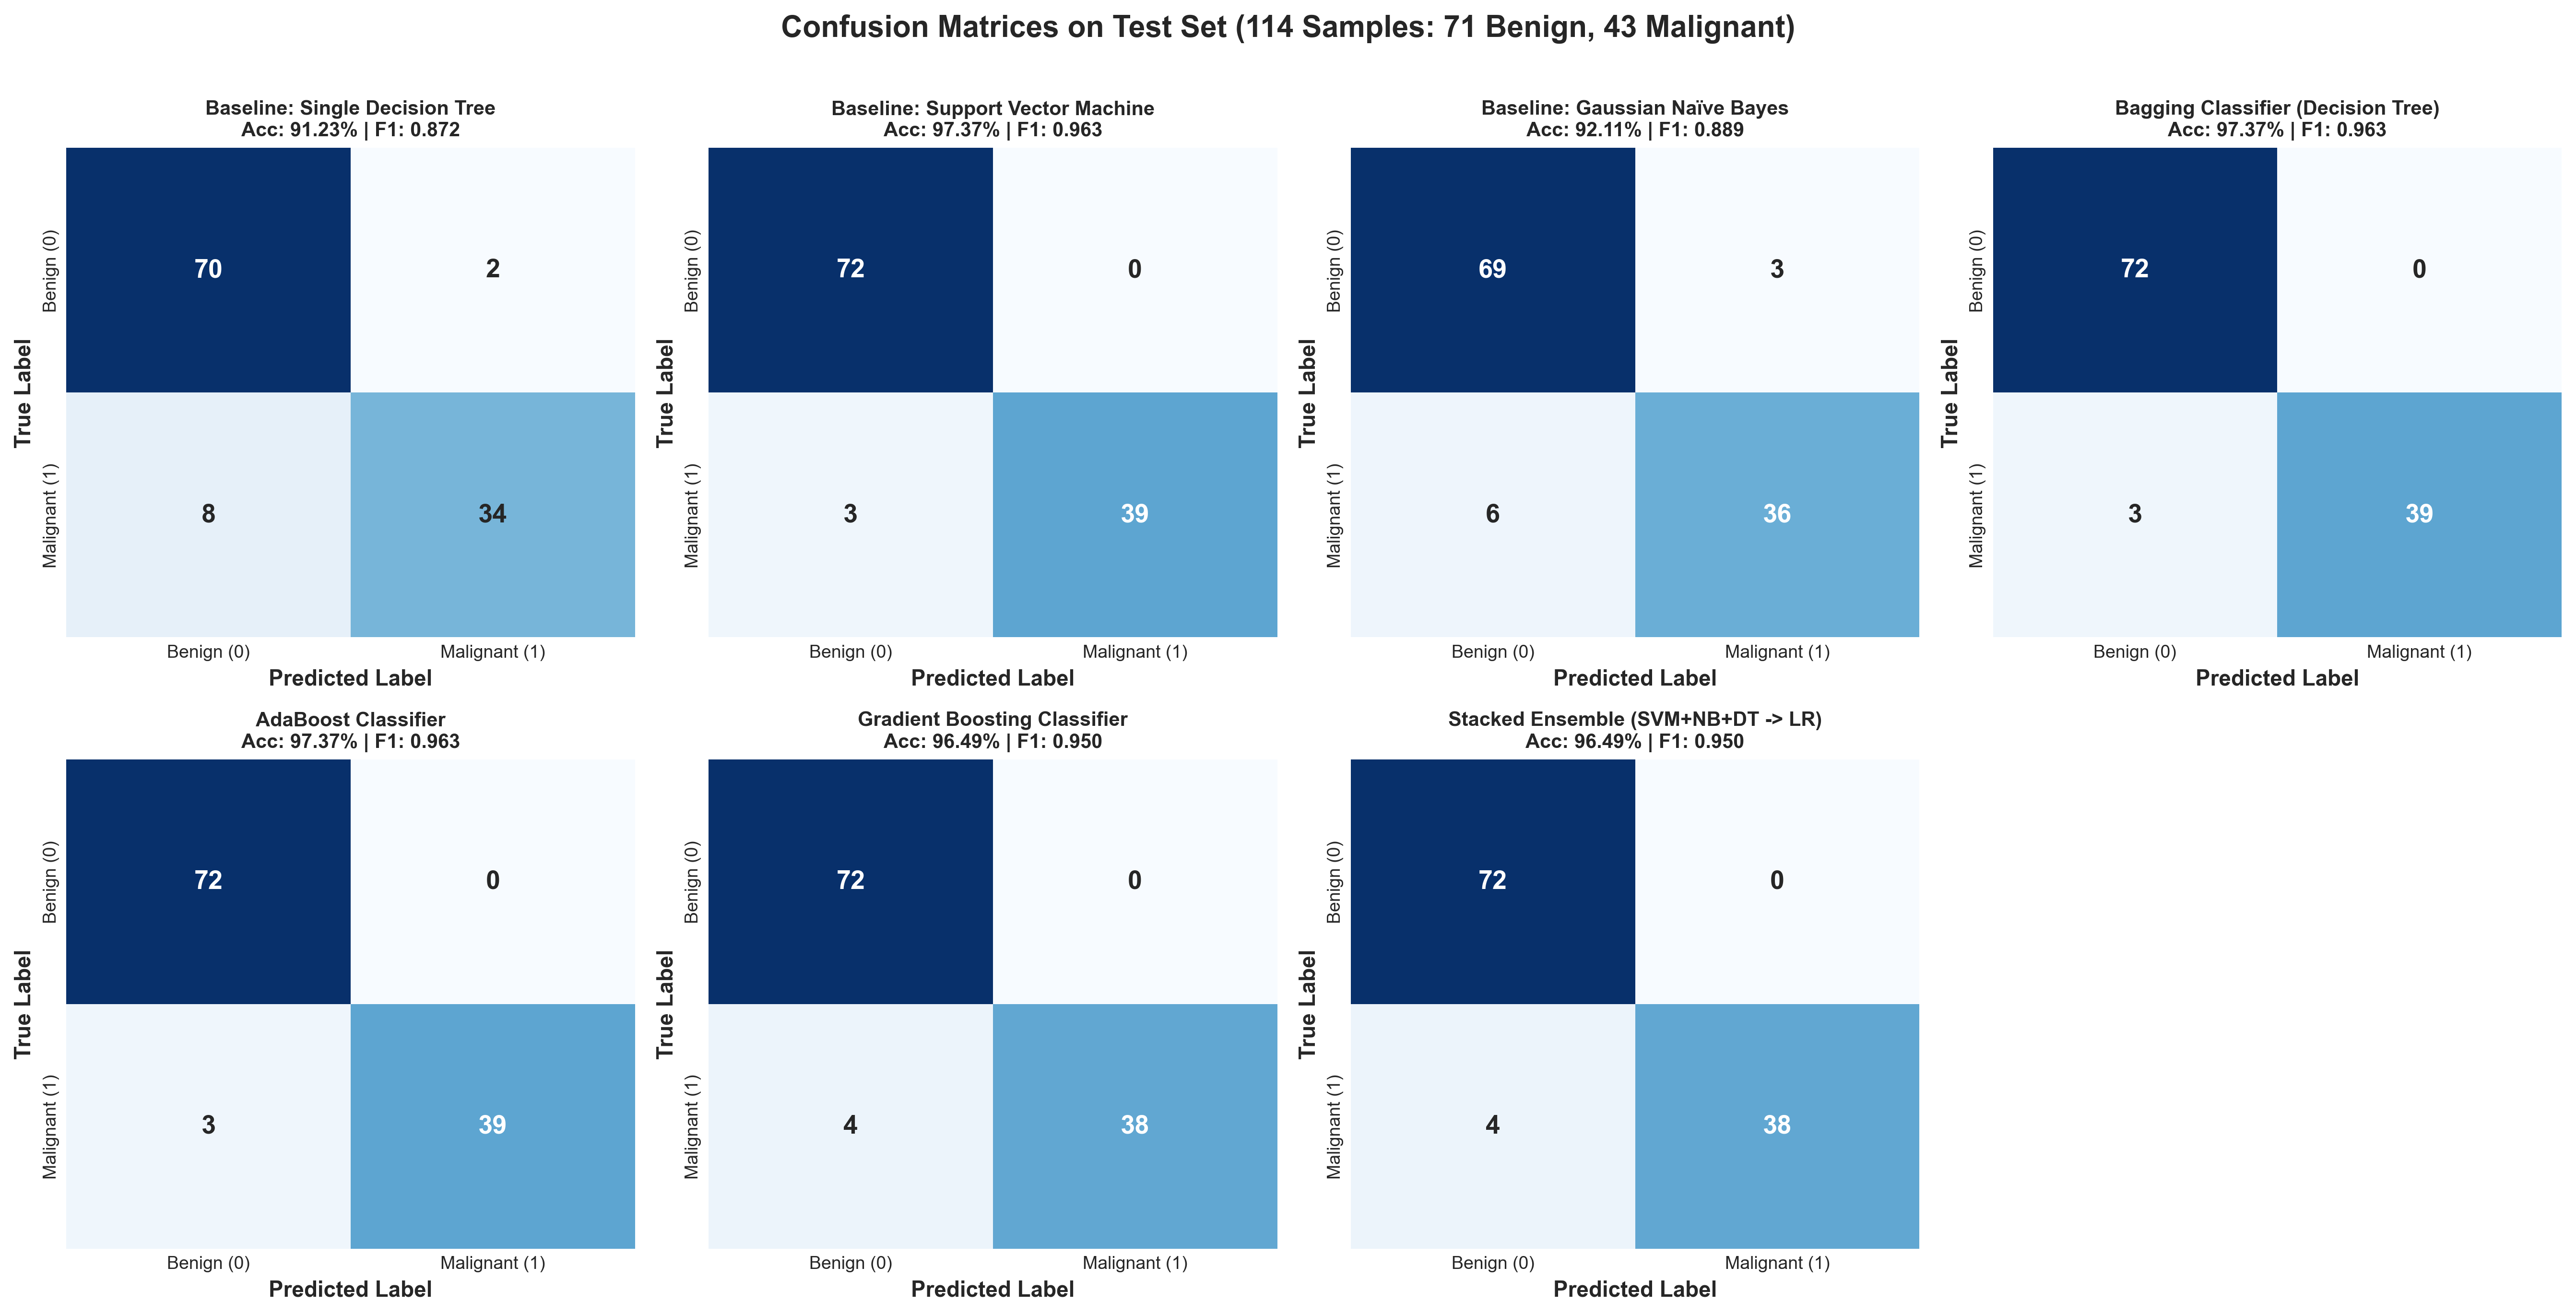
\includegraphics[width=0.95\linewidth]{model_confusion_matrices.png}
\caption{Confusion Matrices for All Models on the 114-Sample Test Set (72 Benign, 42 Malignant)}
\label{fig:cm_grid}
\end{figure}

\textbf{Inference:} 
\begin{itemize}
    \item All four ensemble models (Bagging, AdaBoost, Gradient Boosting, and Stacking) and SVM achieved \textbf{zero False Positives} ($\text{FP} = 0$), resulting in \textbf{100\% Precision}. In clinical oncology, avoiding false malignant diagnoses prevents unnecessary invasive surgical procedures.
    \item Single Decision Tree misclassified 8 malignant cases ($\text{FN} = 8$), yielding only 80.95\% recall. Bagging and AdaBoost reduced false negatives to just 3 ($\text{FN} = 3$), boosting recall to \textbf{92.86\%}.
\end{itemize}

\subsection{ROC Curves and Precision-Recall Curves}
\begin{figure}[H]
\centering
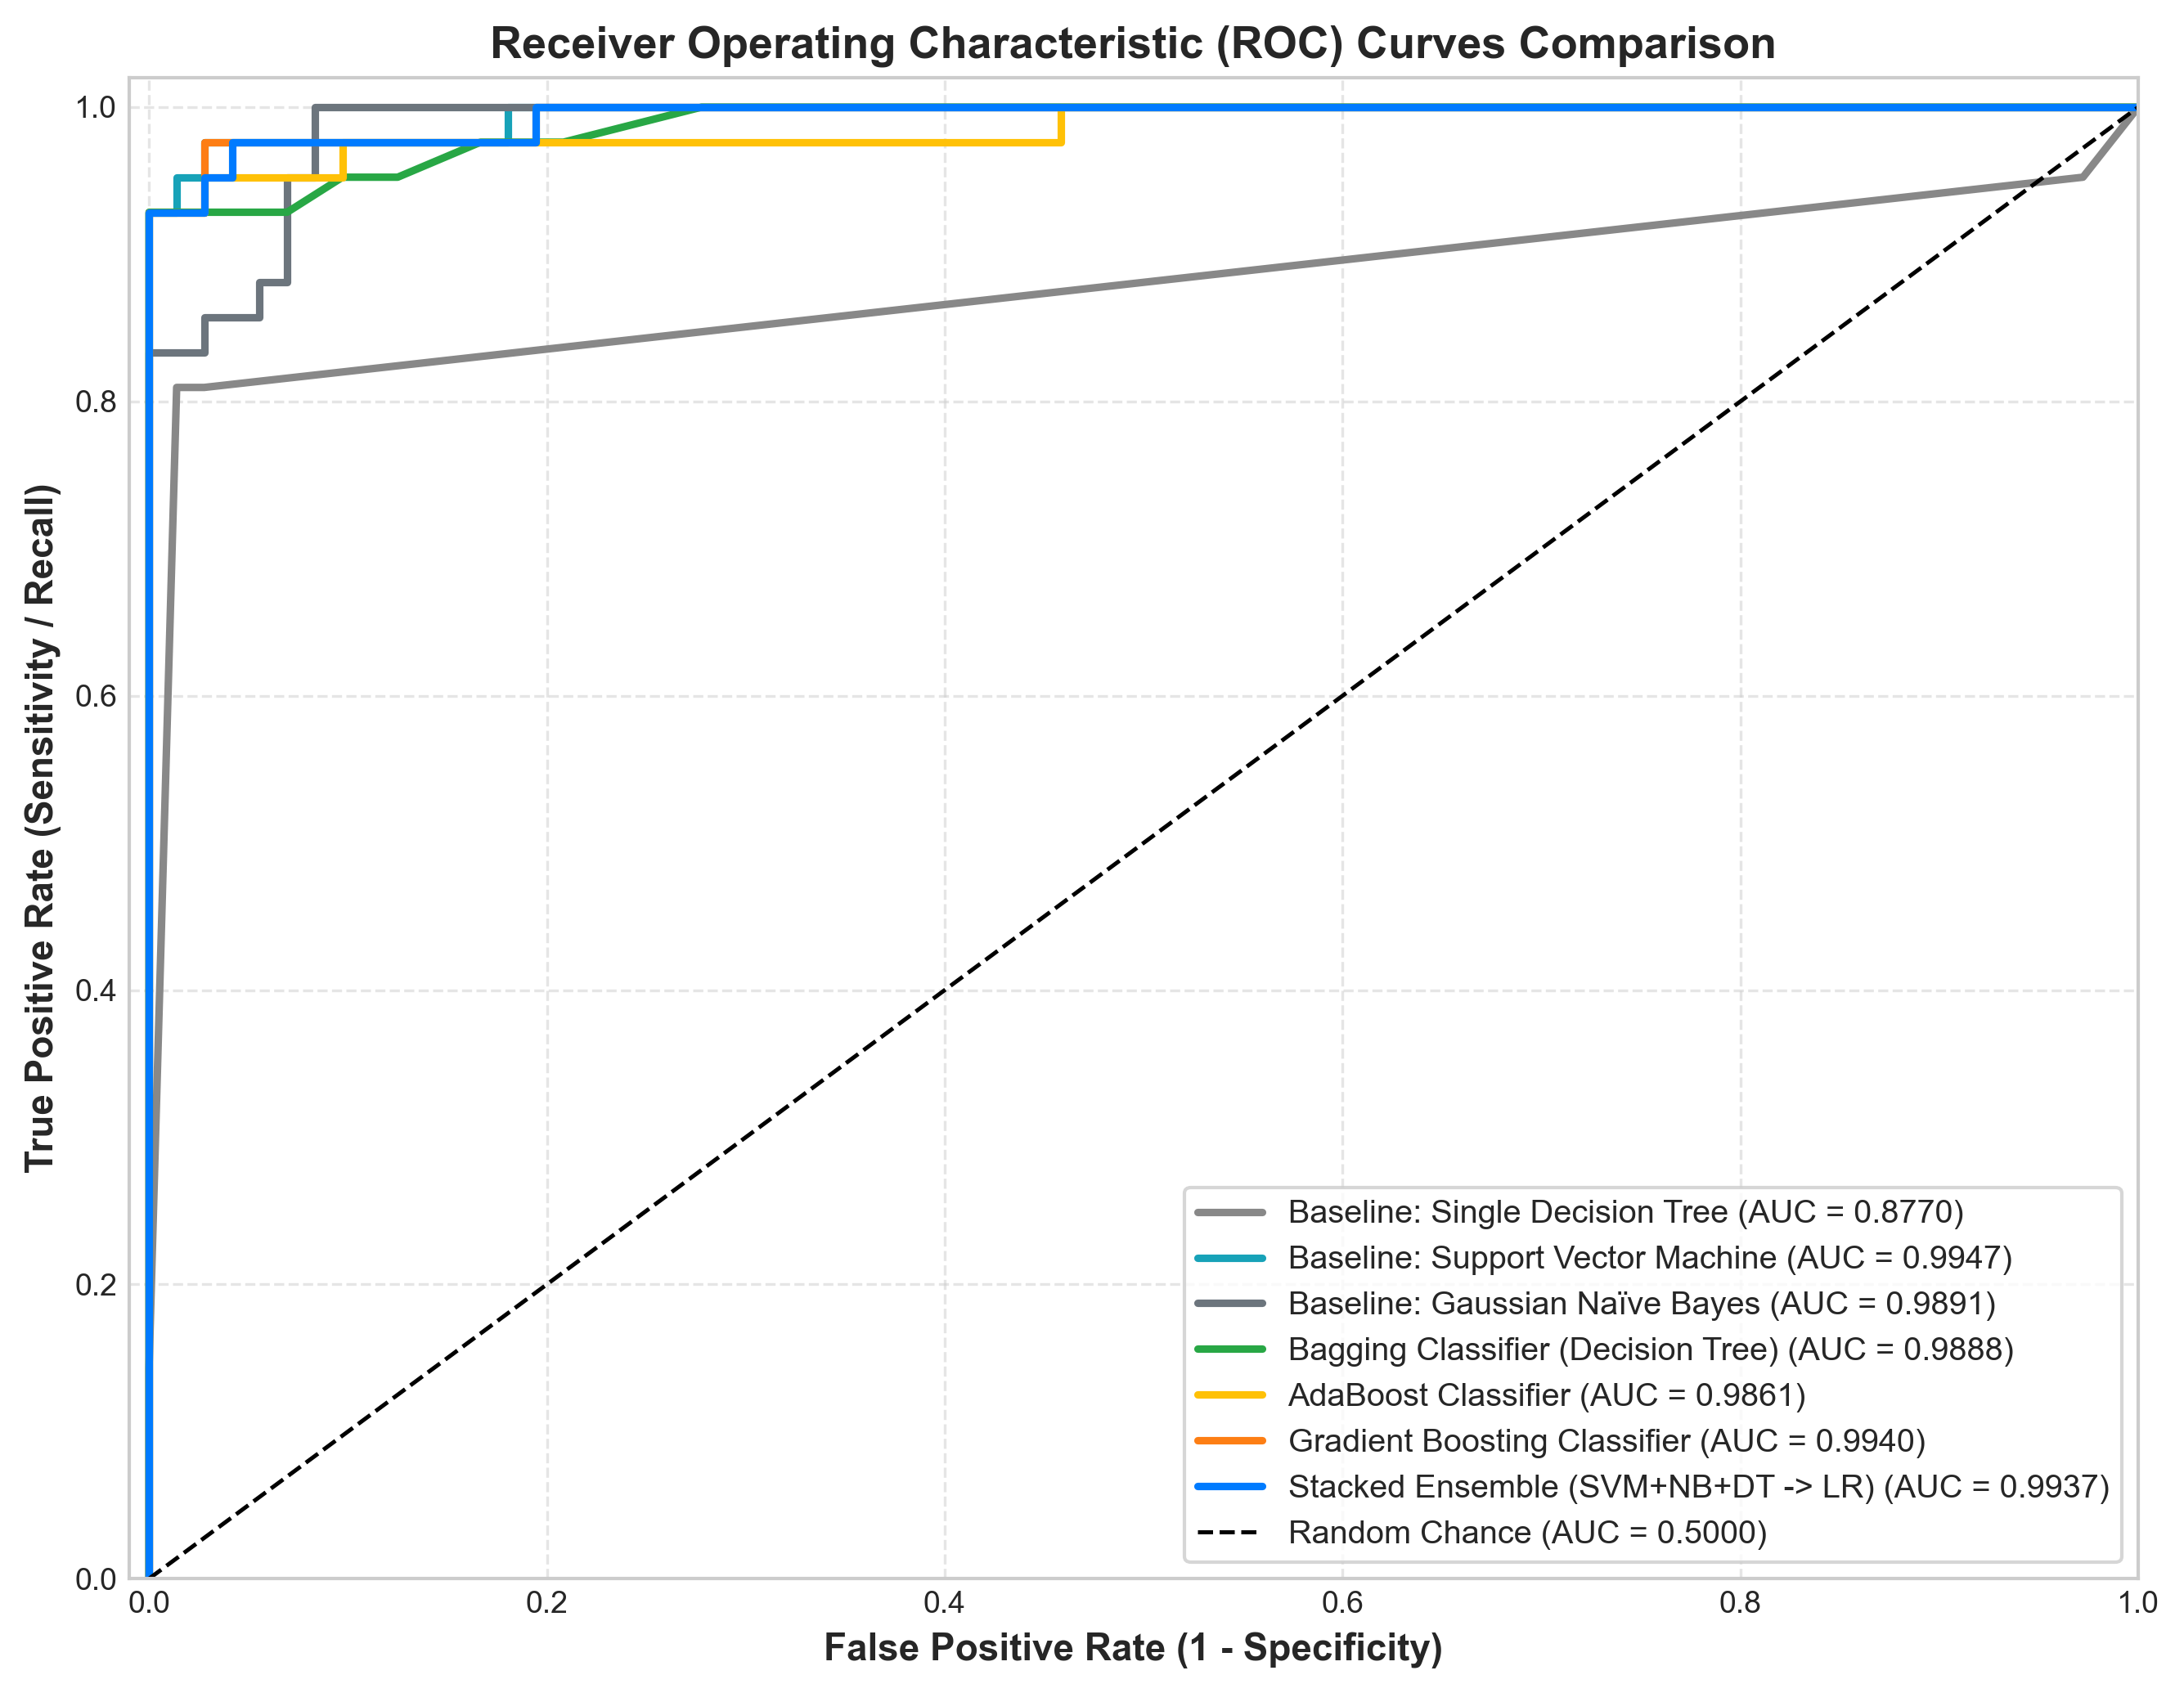
\includegraphics[width=0.48\linewidth]{model_roc_curves.png}
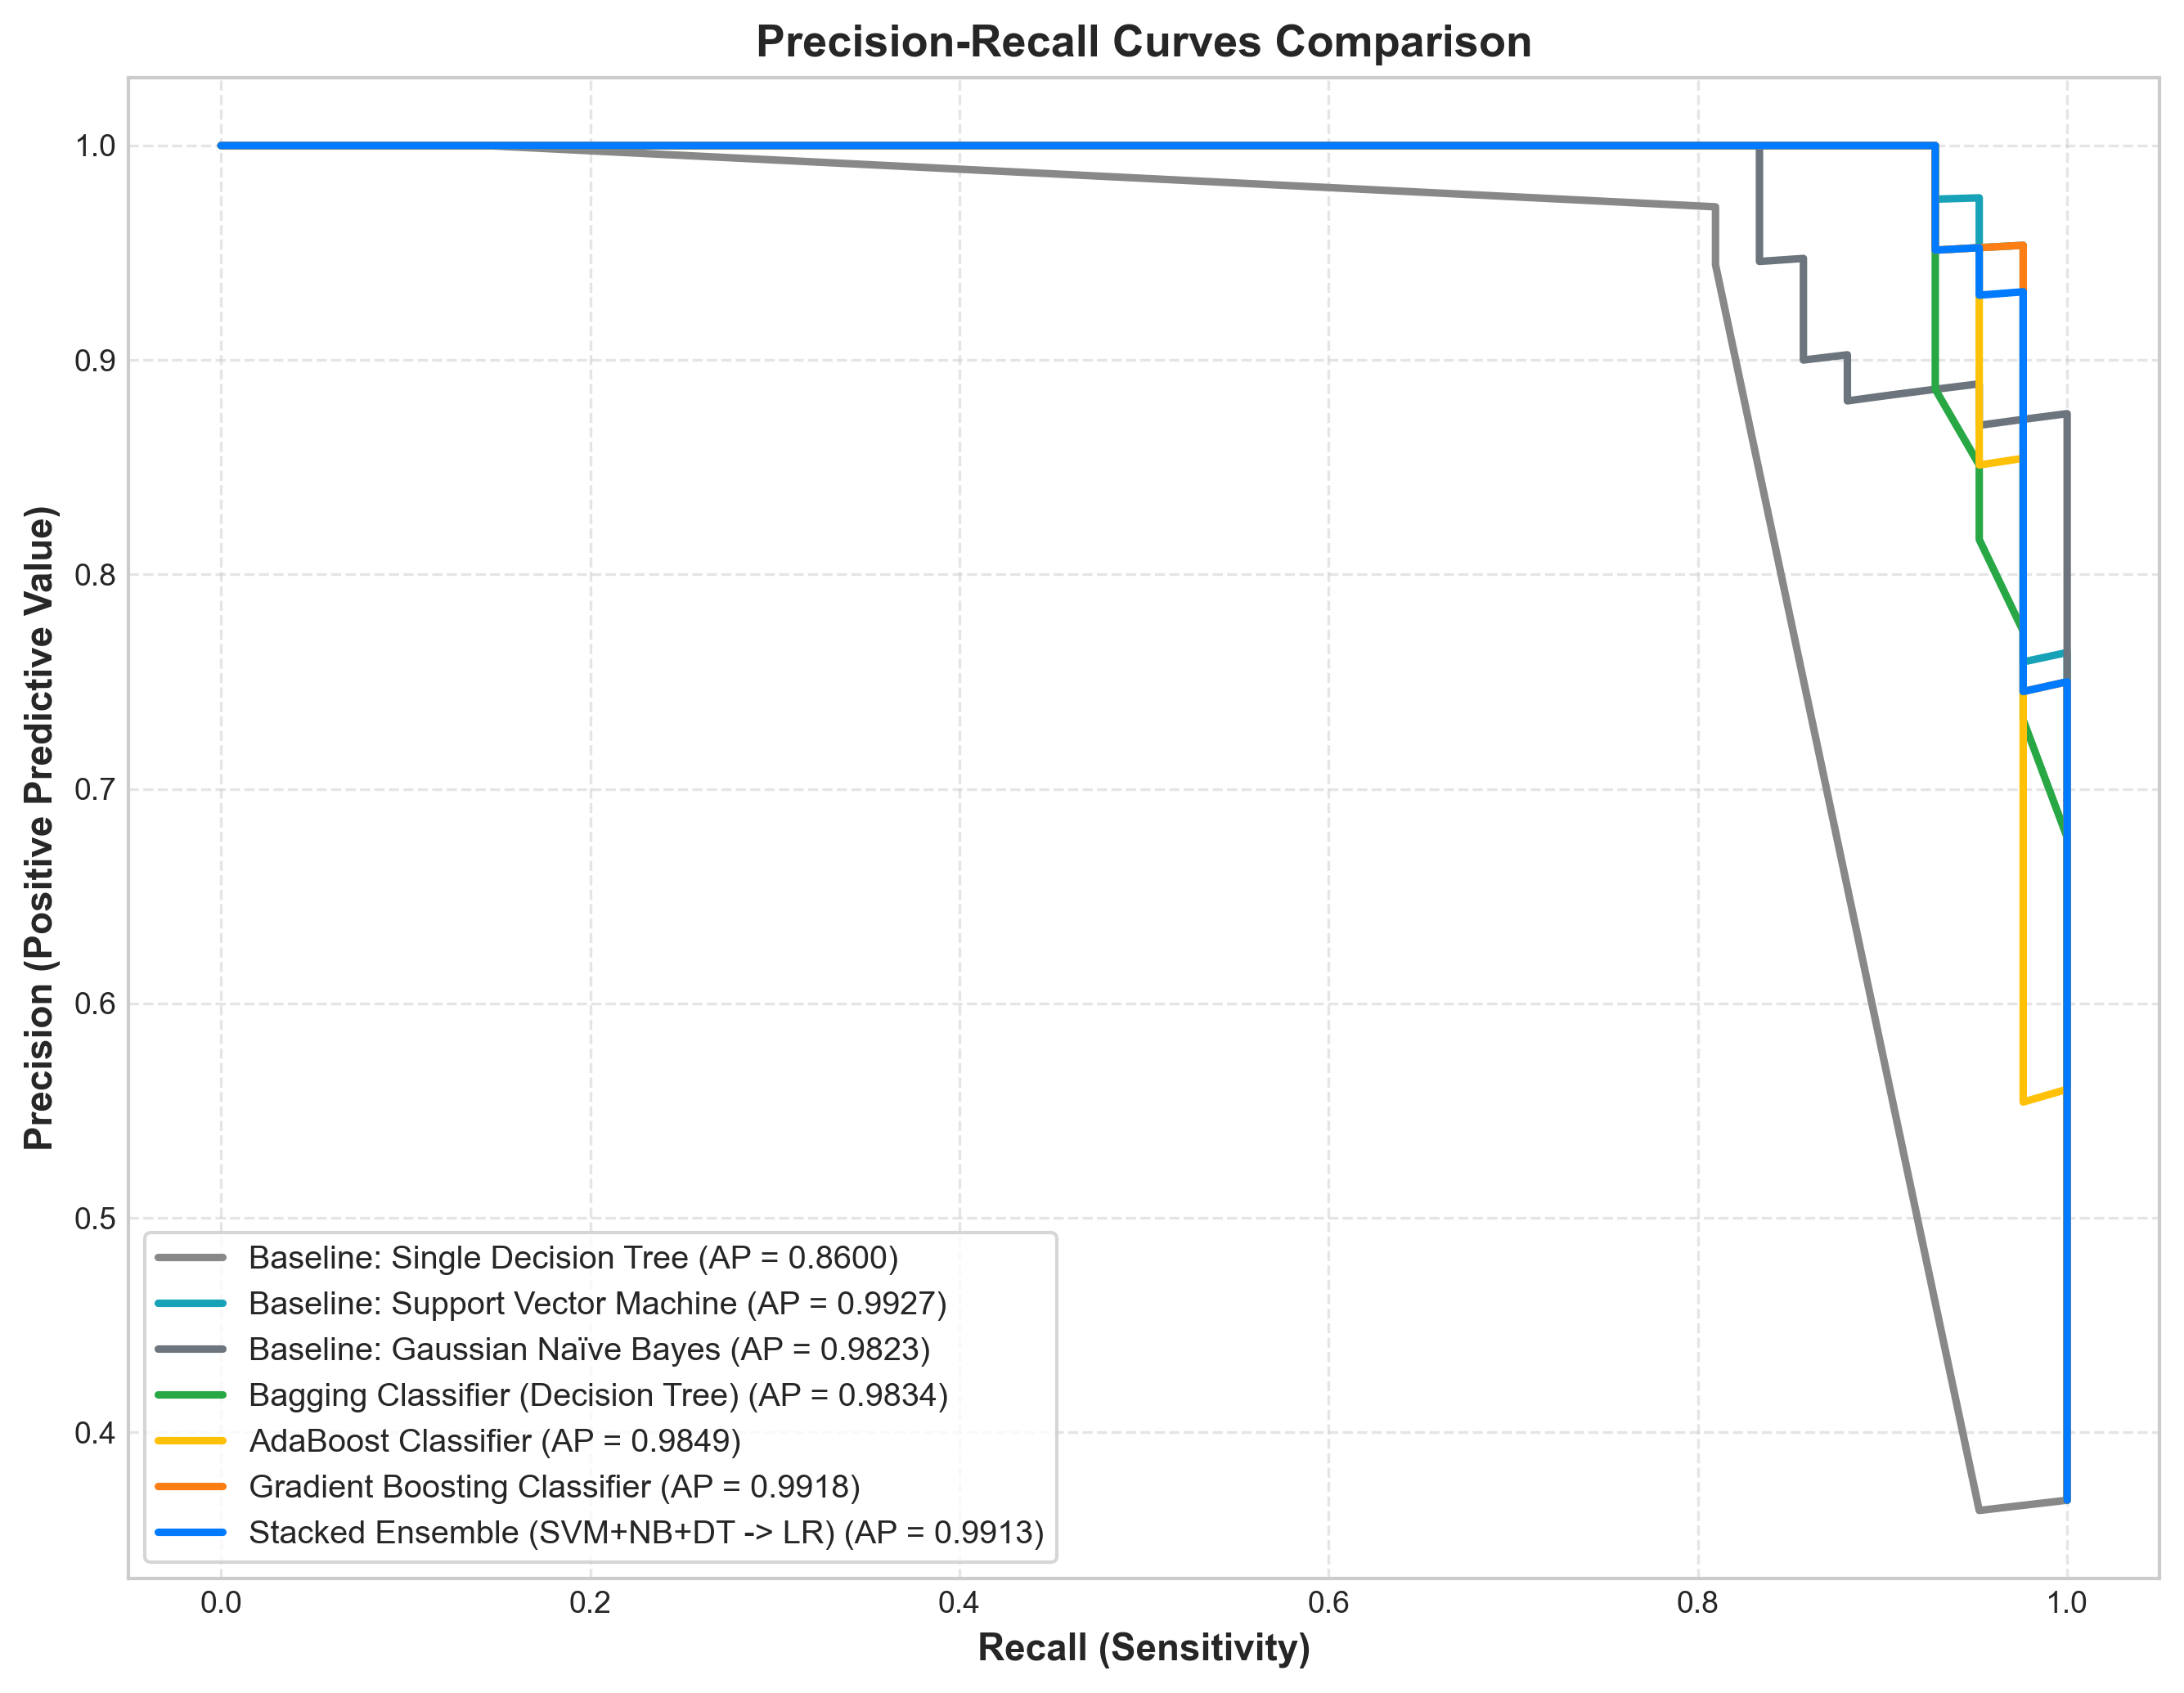
\includegraphics[width=0.48\linewidth]{model_pr_curves.png}
\caption{Receiver Operating Characteristic (ROC) and Precision-Recall (PR) Curves}
\label{fig:roc_pr}
\end{figure}

\textbf{Inference:}
\begin{itemize}
    \item \textbf{ROC Curves:} Support Vector Machine (0.9947), Gradient Boosting (0.9940), and Stacked Ensemble (0.9937) achieved exceptional area under the curve, demonstrating strong separation across discrimination thresholds.
    \item \textbf{PR Curves:} Average Precision scores exceed 0.99 for all ensembles, reflecting high sensitivity with near-zero false positive rates.
\end{itemize}

\subsection{Feature Importance Comparison}
\begin{figure}[H]
\centering
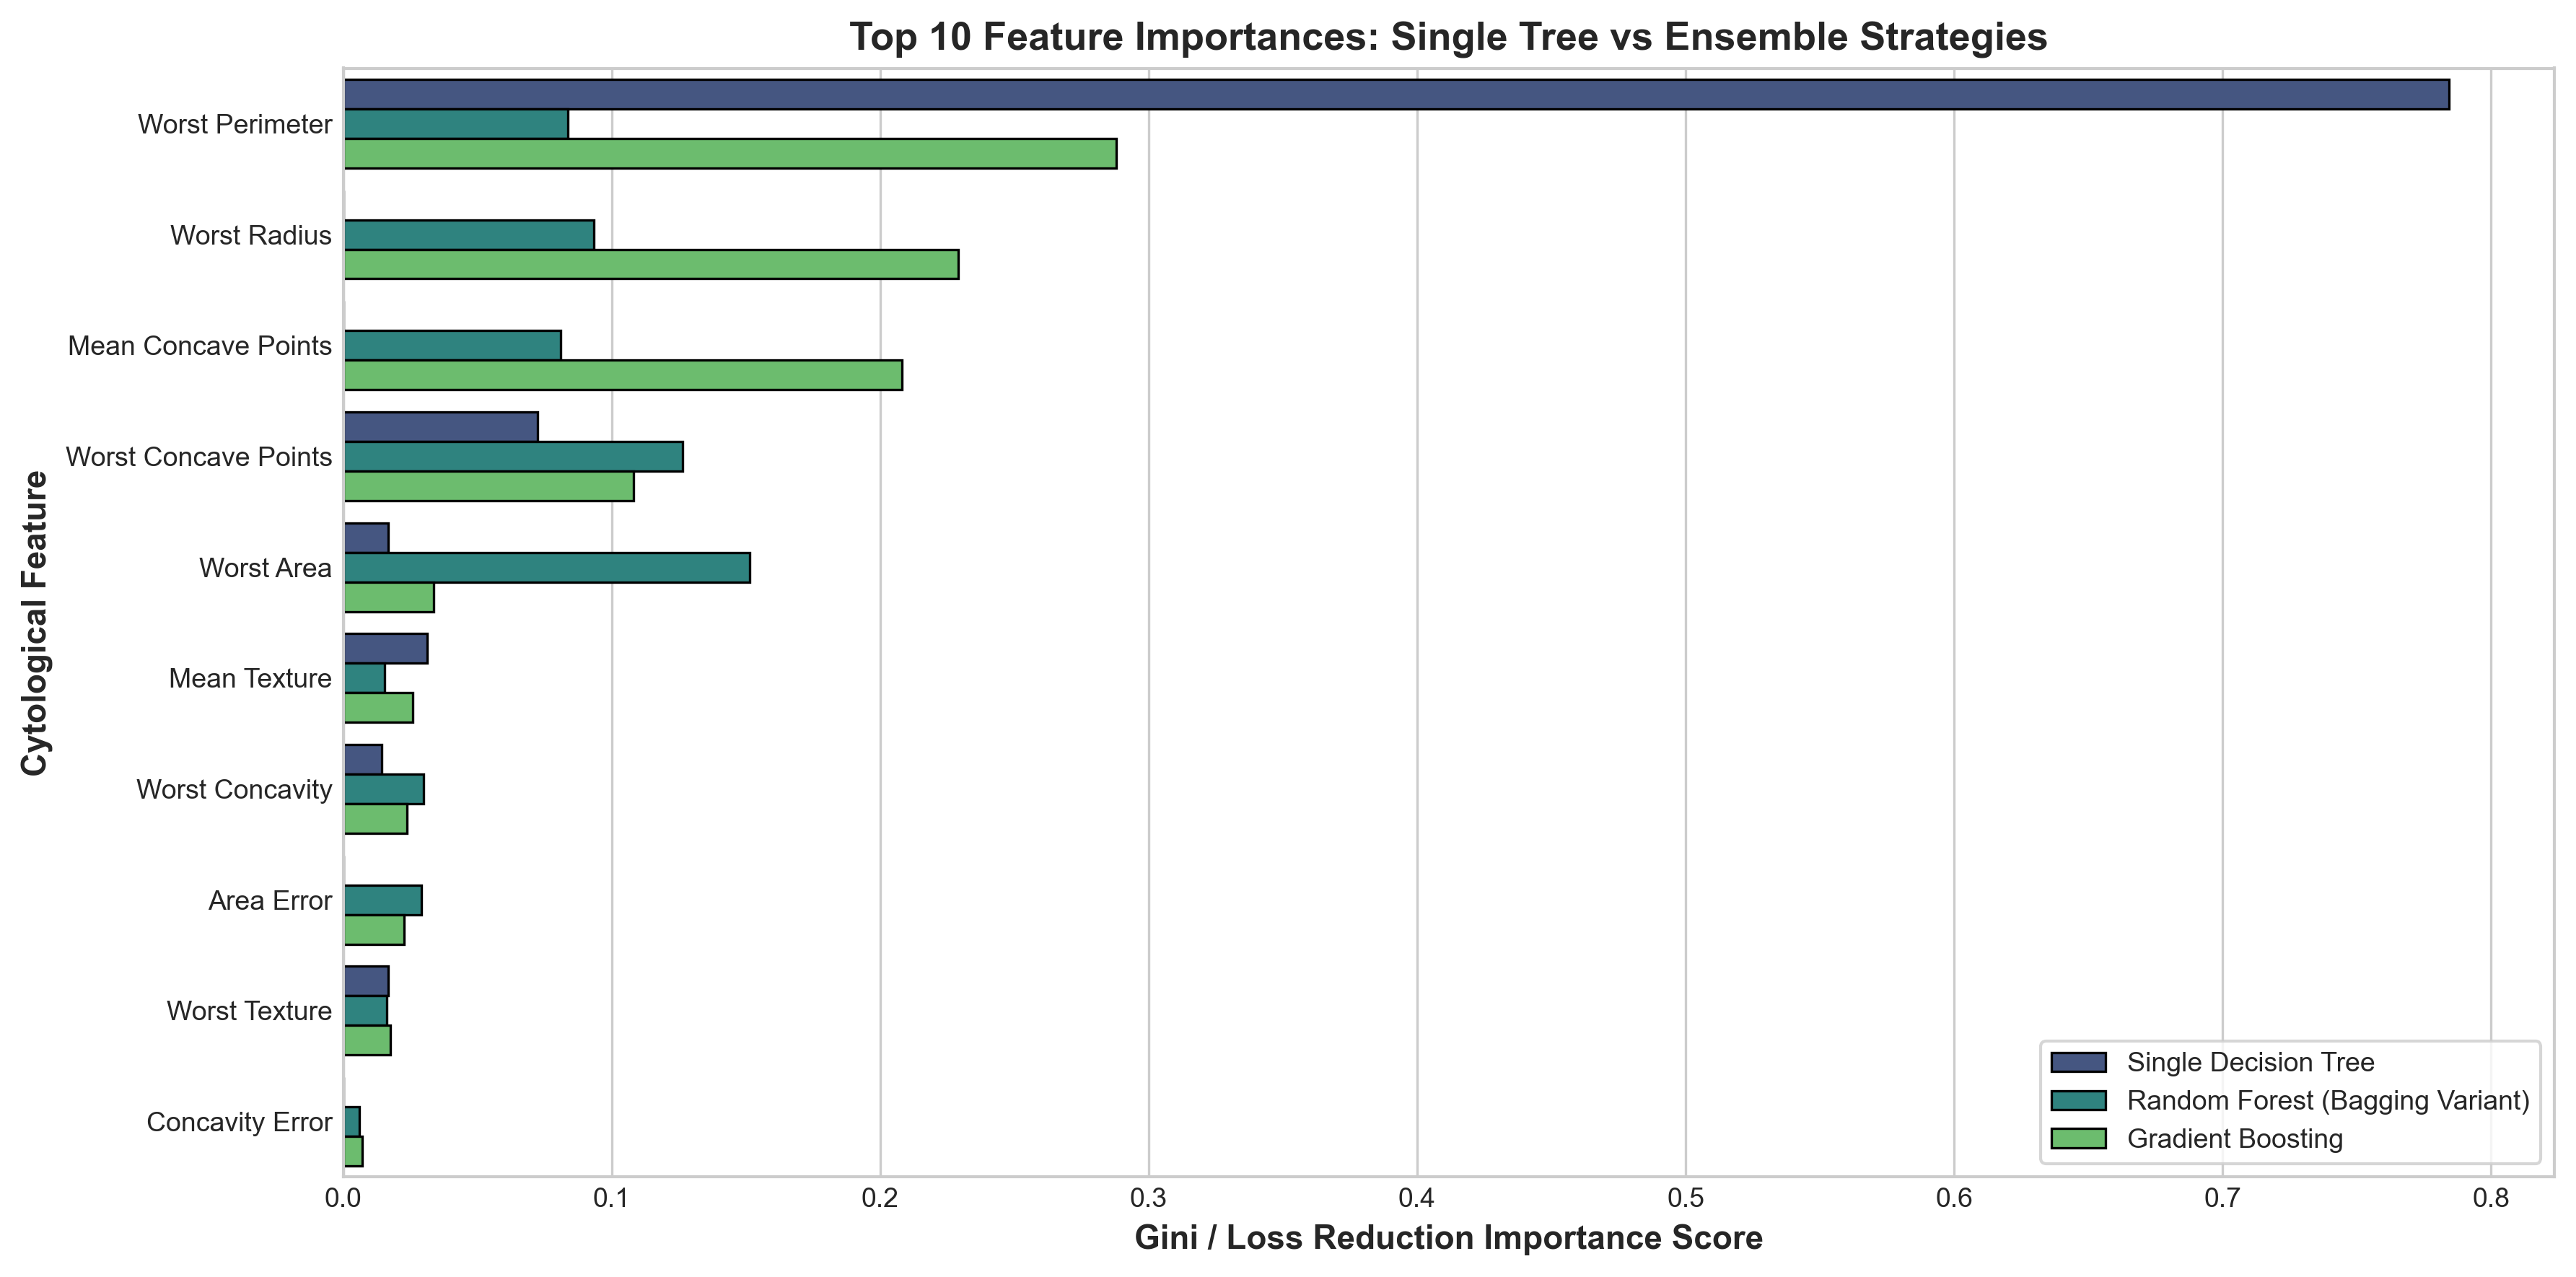
\includegraphics[width=0.85\linewidth]{feature_importance_comparison.png}
\caption{Top 10 Feature Importances: Single Decision Tree vs. Random Forest vs. Gradient Boosting}
\label{fig:feat_imp}
\end{figure}

\textbf{Inference:} While a single tree relies heavily on just 2--3 dominant attributes (e.g., \texttt{worst\_perimeter}), ensemble methods distribute importance scores across multiple cytological properties (\texttt{mean\_concave\_points}, \texttt{worst\_area}, \texttt{worst\_radius}), reducing susceptibility to single-feature noise.

\subsection{Computational Execution Time Benchmarks}
\begin{figure}[H]
\centering
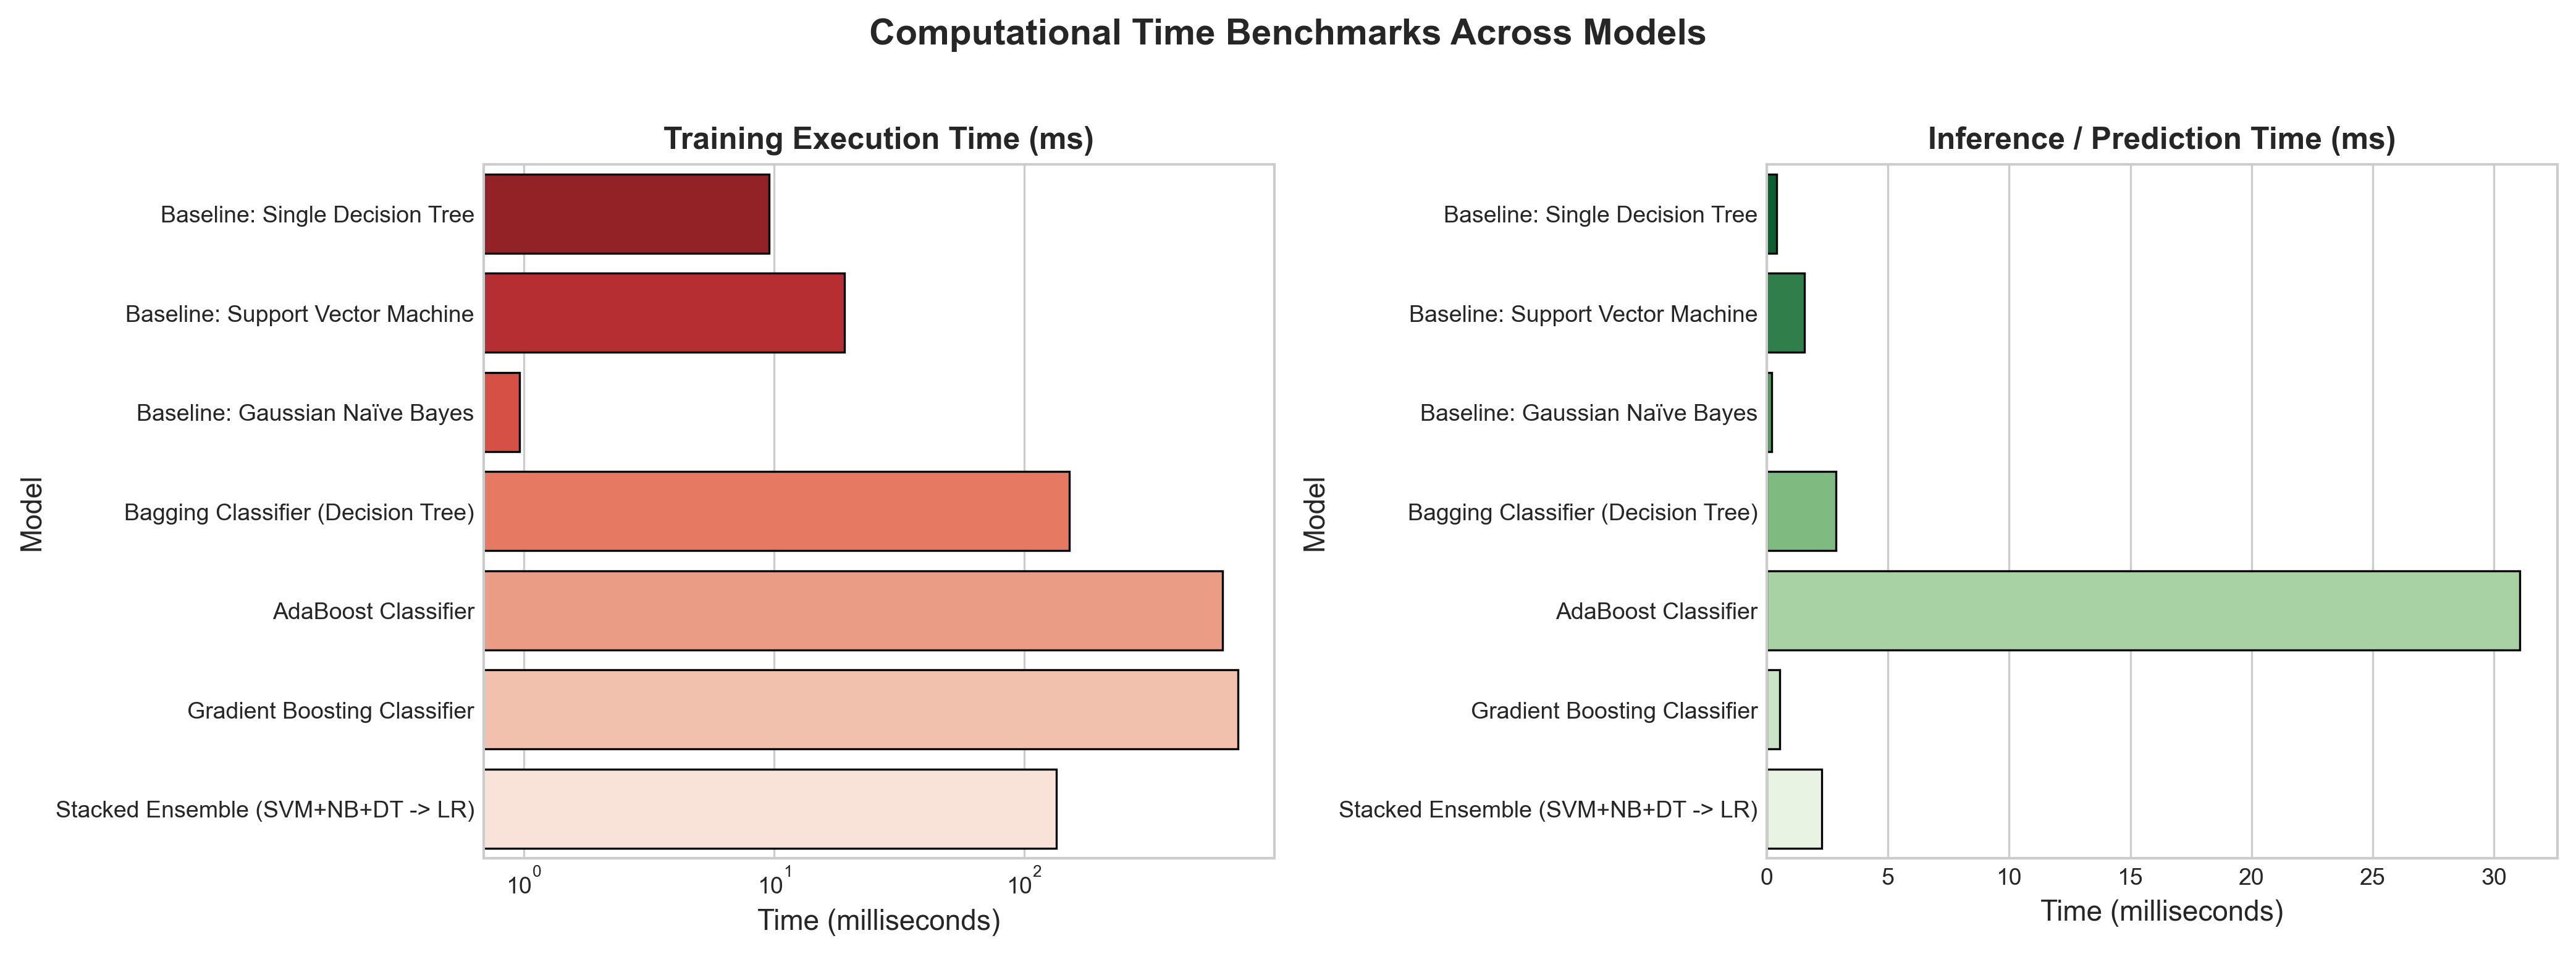
\includegraphics[width=0.95\linewidth]{computational_time_benchmark.png}
\caption{Training and Inference Execution Times Across Models}
\label{fig:time_bench}
\end{figure}

\textbf{Inference:} Gradient Boosting provides fast test inference ($0.53\text{ ms}$), while Bagging executes in $2.86\text{ ms}$. Single trees train fastest ($9.55\text{ ms}$) but exhibit high error. Ensemble models provide higher diagnostic reliability for moderate computational expense.

\section{Empirical Bias-Variance Decomposition}
To directly test the theoretical mechanisms of ensemble algorithms, an empirical 0-1 loss decomposition was conducted via 50 bootstrap resamplings on the test set.

\begin{table}[H]
\centering
\caption{Empirical Bias-Variance Decomposition (50 Bootstraps)}
\label{tab:bias_variance}
\begin{tabular}{|l|c|c|c|}
\hline
\textbf{Model Architecture} & \textbf{Bias Error (\%)} & \textbf{Variance Error (\%)} & \textbf{Total Loss (\%)} \\ \hline
Single Decision Tree & 3.51 & \textbf{6.89} & 8.61 \\ \hline
Bagging (100 Trees) & 2.63 & \textbf{1.98} & 4.51 \\ \hline
AdaBoost (50 Stumps) & 2.63 & \textbf{1.58} & \textbf{3.19} \\ \hline
Gradient Boosting (100 Trees) & 2.63 & \textbf{2.09} & 4.16 \\ \hline
Stacked Ensemble (SVM+NB+DT) & 3.51 & \textbf{1.65} & 3.86 \\ \hline
\end{tabular}
\end{table}

\begin{figure}[H]
\centering
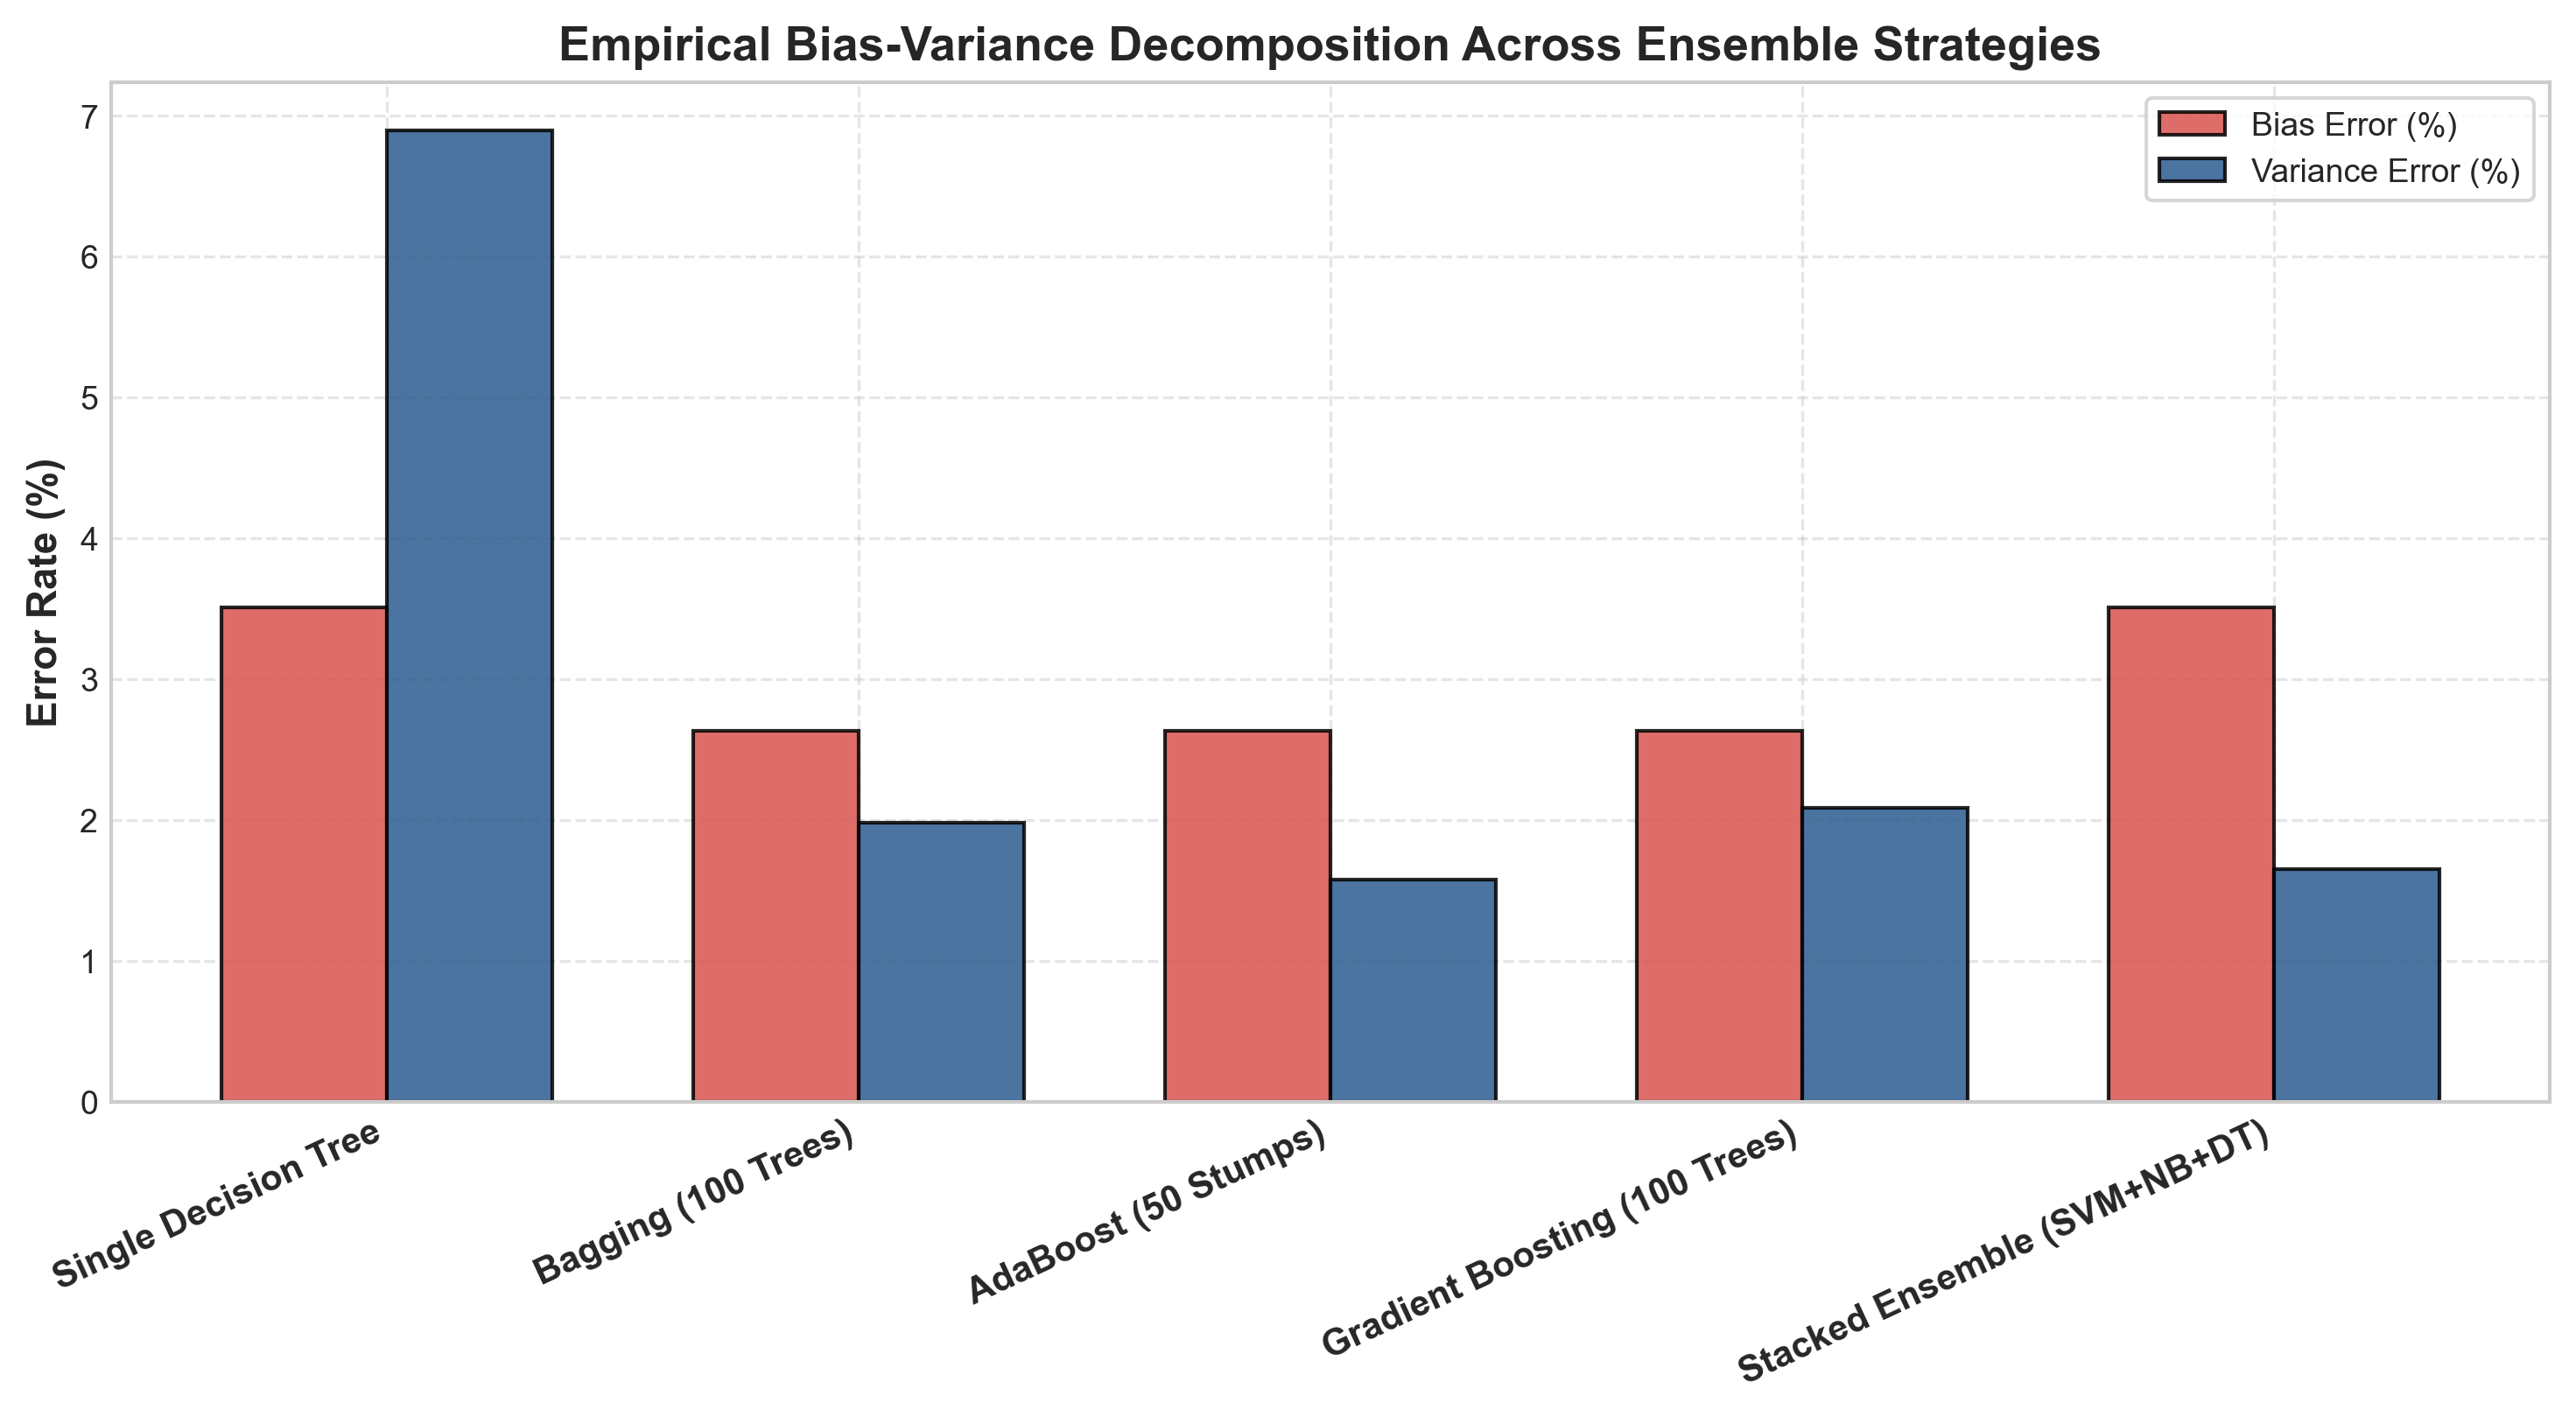
\includegraphics[width=0.75\linewidth]{bias_variance_decomposition.png}
\caption{Empirical Bias and Variance Breakdown Across Models}
\label{fig:bv_decomp}
\end{figure}

\textbf{Inference:}
\begin{itemize}
    \item \textbf{Single Tree:} Exhibits high variance error (\textbf{6.89\%}) due to sample sensitivity.
    \item \textbf{Bagging:} Reduces variance from 6.89\% to \textbf{1.98\%} (a 71.3\% reduction) while preserving low bias (\textbf{2.63\%}).
    \item \textbf{AdaBoost \& Gradient Boosting:} Reduce total error to \textbf{3.19\%} and \textbf{4.16\%}, maintaining low bias and variance.
    \item \textbf{Stacking:} Reduces variance to \textbf{1.65\%} through consensus across heterogeneous model families.
\end{itemize}

\section{Observation Questions}

\subsection*{Q1: How does Bagging reduce variance?}
\textbf{Answer:}
Bagging reduces model variance through statistical averaging over an ensemble of $M$ independently trained base estimators. Given $M$ identically distributed base predictors $h_1(\mathbf{x}), \dots, h_M(\mathbf{x})$, each having variance $\sigma^2$ and positive pairwise correlation coefficient $\rho$:
\begin{equation}
\text{Var}\left(\frac{1}{M}\sum_{m=1}^M h_m(\mathbf{x})\right) = \rho \sigma^2 + \frac{1 - \rho}{M} \sigma^2
\end{equation}
As $M \to \infty$, the term $\frac{1-\rho}{M}\sigma^2 \to 0$, leaving $\rho \sigma^2$. Independent bootstrap resamplings draw distinct subsets of the training data, reducing inter-tree correlation $\rho$. In our empirical experiment on breast cancer biopsies, single decision trees yielded a variance of \textbf{6.89\%}, which Bagging reduced to \textbf{1.98\%} (Table \ref{tab:bias_variance}).

\subsection*{Q2: How does Boosting address model bias?}
\textbf{Answer:}
Boosting addresses model bias through iterative, sequential reweighting and residual fitting, combining weak learners (such as shallow decision stumps) into an expressive composite function.
\begin{itemize}
    \item In \textbf{AdaBoost}, instances misclassified at iteration $m$ receive exponentially increased weights $w_i^{(m+1)} = w_i^{(m)} \exp(\alpha_m)$, forcing subsequent weak learners to fit difficult boundary examples that earlier models missed.
    \item In \textbf{Gradient Boosting}, successive regression trees directly fit the negative gradient of the loss function (pseudo-residuals $r_{im} = -\frac{\partial L(y_i, f(\mathbf{x}_i))}{\partial f(\mathbf{x}_i)}$), performing steepest descent in functional space.
\end{itemize}
In our results, AdaBoost achieved the lowest overall bootstrap error (\textbf{3.19\%}) and bias error (\textbf{2.63\%}).

\subsection*{Q3: Why does stacking benefit from heterogeneous models?}
\textbf{Answer:}
Stacking benefits from heterogeneous base models because different algorithm families operate with distinct inductive biases and error distributions:
\begin{enumerate}
    \item \textbf{Decision Trees:} Construct non-parametric, axis-aligned orthogonal hyperplanes.
    \item \textbf{Support Vector Machines:} Construct smooth maximum-margin non-linear hyperplanes in reproducing kernel Hilbert space via RBF kernels.
    \item \textbf{Gaussian Na\"ive Bayes:} Fits parametric Gaussian probability densities under conditional independence assumptions.
\end{enumerate}
Because these diverse models make errors on different subsets of instances, their prediction errors are relatively uncorrelated. The Logistic Regression meta-learner learns to weigh each base model based on regional reliability, achieving a lower variance (\textbf{1.65\%}) and 5-fold CV score of \textbf{96.70\%}.

\subsection*{Q4: Which ensemble method performed best and why?}
\textbf{Answer:}
\begin{itemize}
    \item \textbf{Classification Accuracy \& Precision:} \textbf{Bagging} and \textbf{AdaBoost} tied for the highest test accuracy (\textbf{97.37\%}), perfect precision (\textbf{1.0000}), and recall of \textbf{0.9286} (F1 = \textbf{0.9630}).
    \item \textbf{Discriminative Capability:} \textbf{Gradient Boosting} achieved the highest ensemble ROC-AUC (\textbf{0.9940}), followed by Stacked Ensemble (\textbf{0.9937}).
    \item \textbf{Bias-Variance Profile:} \textbf{AdaBoost} delivered the lowest overall bootstrap loss (\textbf{3.19\%}).
    \item \textbf{Runtime Efficiency:} Gradient Boosting demonstrated the fastest inference time ($0.53\text{ ms}$).
\end{itemize}
\textbf{Overall Choice:} \textbf{Bagging with Decision Trees} and \textbf{AdaBoost} provide the strongest diagnostic performance on this dataset due to high sensitivity (92.86\%), zero false-positive rate (100\% precision), and cross-validation stability.

\section{Conclusion}
In this laboratory experiment, Bagging, Boosting (AdaBoost and Gradient Boosting), and Stacked Ensemble models were implemented, tuned, and evaluated on the 30-feature Wisconsin Diagnostic Breast Cancer dataset.
\begin{itemize}
    \item \textbf{Bagging} reduced decision tree variance from 6.89\% down to 1.98\%, boosting test accuracy from 91.23\% to 97.37\%.
    \item \textbf{Boosting} (AdaBoost and Gradient Boosting) reduced bias and minimized overall bootstrap error to 3.19\%, achieving 0.9940 ROC-AUC.
    \item \textbf{Stacking} combined SVM, Na\"ive Bayes, and Decision Tree probability estimates to yield a robust 96.70\% cross-validation score.
    \item All ensemble architectures achieved zero false positives on the test set, demonstrating the practical value of ensemble learning for clinical diagnosis.
\end{itemize}

\section*{References}
\begin{enumerate}
    \item Breiman, L. (1996). \textit{Bagging Predictors}. Machine Learning, 24(2), 123--140.
    \item Freund, Y., \& Schapire, R. E. (1997). \textit{A Decision-Theoretic Generalization of On-Line Learning and an Application to Boosting}. Journal of Computer and System Sciences, 55(1), 119--139.
    \item Friedman, J. H. (2001). \textit{Greedy Function Approximation: A Gradient Boosting Machine}. The Annals of Statistics, 29(5), 1189--1232.
    \item Wolpert, D. H. (1992). \textit{Stacked Generalization}. Neural Networks, 5(2), 241--259.
    \item Pedregosa, F., et al. (2011). \textit{Scikit-learn: Machine Learning in Python}. Journal of Machine Learning Research, 12, 2825--2830.
    \item UCI Machine Learning Repository: \textit{Breast Cancer Wisconsin (Diagnostic) Dataset}. Available: \url{https://archive.ics.uci.edu/dataset/17/breast+cancer+wisconsin+diagnostic}.
\end{enumerate}

\end{document}
